%%%%% Single page layout:
%%%%% -----------------------------------
\newcommand{\singlePage}{
	\documentclass[12pt, a4paper]{report}
	\setlength\textwidth{145mm}
	\setlength\textheight{247mm}
	\setlength\oddsidemargin{15mm}
	\setlength\evensidemargin{15mm}
	\setlength\topmargin{0mm}
	\setlength\headsep{0mm}
	\setlength\headheight{0mm}
	\let\openright=\clearpage
}


%%%%% Double page layout
%%%%% -----------------------------------
\newcommand{\doublePage}{
	\documentclass[12pt, a4paper, twoside, openright]{report}
	\setlength\textwidth{145mm}
	\setlength\textheight{247mm}
	\setlength\oddsidemargin{15mm}
	\setlength\evensidemargin{0mm}
	\setlength\topmargin{0mm}
	\setlength\headsep{0mm}
	\setlength\headheight{0mm}
	\let\openright=\cleardoublepage
}

%\singlePage
\doublePage


%%% Additional useful packages
%%% ----------------------------------------------------------------
\usepackage{amsmath}        
\usepackage{amsfonts}       
\usepackage{amsthm}         
\usepackage{bm}             
\usepackage{graphicx}       
%\usepackage{psfrag}         
\usepackage{fancyvrb}       
\usepackage{natbib}         
%\usepackage[round]{natbib}         
\usepackage{bbding}         
\usepackage{dcolumn}        
\usepackage{booktabs}       
\usepackage{paralist}       
%\usepackage{indentfirst}    
\usepackage[nottoc]{tocbibind}
\usepackage[mathscr]{euscript}
\usepackage{epstopdf}
\usepackage[small,labelfont=bf,up,textfont=up]{caption, subcaption}
%\usepackage{subcaption}
\usepackage{multirow,tabularx}
\usepackage[utf8]{inputenc}
\usepackage{color}
%\usepackage{trackchanges}
\usepackage{mathtools}
\usepackage{xfrac}
%\usepackage{tabulary}
\usepackage{tikz}
%\usepackage{showframe}
\usepackage[unicode]{hyperref}
\usepackage{rotating}

\usepackage{lipsum}

%\overfullrule=1mm

\usepackage{floatrow}
\DeclareFloatFont{tableFontSize}{\small}% "scriptsize" is defined by floatrow, "tiny" not
\floatsetup[table]{font=tableFontSize}

\usepackage{listings} % include R scripts (and other)
\lstset{
	language=R,
	basicstyle=\scriptsize\ttfamily,
	commentstyle=\ttfamily\color{gray},
	numbers=left,
	numberstyle=\ttfamily\color{gray}\footnotesize,
	stepnumber=1,
	numbersep=5pt,
	backgroundcolor=\color{white},
	showspaces=false,
	showstringspaces=false,
	showtabs=false,
	frame=single,
	tabsize=2,
	captionpos=b,
	breaklines=true,
	breakatwhitespace=false,
	title=\lstname,
	escapeinside={},
	keywordstyle={},
	morekeywords={}
}
\newcommand{\includecode}[2]{\lstinputlisting[language=R, caption=#2]{../computations/#1}}
\renewcommand{\lstlistingname}{Script}
\renewcommand{\lstlistlistingname}{List of Scripts}

\hypersetup{pdftitle=Thesis Title, 
            pdfauthor=Name Surname,
            ps2pdf,
            colorlinks=false,
            urlcolor=blue,
            pdfstartview=FitH,
            pdfpagemode=UseOutlines,
            pdfnewwindow,
            breaklinks
          }



%%% Deklarace prikazu
%%% ----------------------------------------------------------------
\newcommand{\FIGDIR}{./figures}    %%% directory containing figures

\theoremstyle{plain}
\newtheorem{theorem}{Theorem}[chapter]
\newtheorem{lemma}[theorem]{Lemma}
\newtheorem{proposition}[theorem]{Proposition}
\newtheorem{corollary}[theorem]{Corollary}

\theoremstyle{plain}
\newtheorem{definition}{Definition}[chapter]
\newtheorem{algorithm}{Algorithm}[chapter]

\theoremstyle{definition}
\newtheorem*{note}{Note}
\newtheorem{example}{Example}[chapter] % \demo
\newtheorem*{notation}{Notation}


\newenvironment{prooooF}{
  \par\medskip\noindent
  \textit{Proeof}.
}{
\newline
\rightline{\square}
}

\newcommand\xqed[1]{%
  \leavevmode\unskip\penalty9999 \hbox{}\nobreak\hfill
  \quad\hbox{#1}}
\newcommand\demo{\xqed{$\triangle$}}




\bibliographystyle{plainnat}     %% Author (year) style
%\bibliographystyle{myplainnat}     %% Author (year) style
%\bibliographystyle{unsrt}        %% [number] style


%%%%% ------------------------------------------------------------
\DefineVerbatimEnvironment{PCinout}{Verbatim}{fontsize=\small, frame=single}

% general sets
\newcommand{\R}{\mathbb{R}}
\newcommand{\N}{\mathbb{N}}

% probability operators
\DeclareMathOperator{\pr}{\mathbb{P}}
\DeclareMathOperator{\E}{\mathbb{E}\,}
\DeclareMathOperator{\var}{\textrm{var}}
\DeclareMathOperator{\sd}{\textrm{sd}}

% functions and constants
\DeclareMathOperator{\e}{\mathrm{e}}
%\DeclareMathOperator{\exp}{\textrm{exp}}

%\newcommand{\m}[1]{\mathbf{#1}}
\newcommand{\m}[1]{\bm{#1}}
\newcommand{\probSpace}{(\Omega ,\, \mathcal{A} ,\, \pr)}
\newcommand{\transSys}{\{ \m{P} (s ,\, t) ,\, t \geq s \geq 0 \}}
\newcommand{\procX}{\m{X} = \{ X_t ,\, t \geq 0 \}}
\newcommand{\proc}[1]{\m{#1} = \{ #1_t ,\, t \geq 0 \}}
\newcommand{\vector}[1]{\bm{#1}}
\newcommand{\Rplus}{[0, \infty)}
\newcommand{\T}[1]{#1^\top}  % transposition of a matrix   

% frequently used matrices
\renewcommand{\x}{\mathbf{x}}
\DeclareMathOperator{\y}{\m{y}}
\DeclareMathOperator{\X}{\m{X}}
\DeclareMathOperator{\z}{\mathbf{z}}
\DeclareMathOperator{\Z}{\m{Z}}
\DeclareMathOperator{\0}{\m{0}}
\renewcommand{\s}{\m{s}}
\renewcommand{\S}{\mathcal{S}}

% statistics
\newcommand{\indexij}{_{Y_{k-1}^{\nu} Y_{k}^{\nu}}}
\newcommand{\indexi}{_{Y_{k-1}^{\nu}}}


% optimization
%\DeclareMathOperator{\max}{\textrm{max}}
%\DeclareMathOperator{\min}{\textrm{min}}
\DeclareMathOperator{\argmax}{\textrm{argmax}}
\DeclareMathOperator{\argmin}{\textrm{argmin}}
\DeclareMathOperator{\st}{\textrm{s.t.}}

\newcommand{\goto}{\rightarrow}
\newcommand{\gotop}{\stackrel{P}{\longrightarrow}}
\newcommand{\gotod}{\stackrel{d}{\longrightarrow}}
\newcommand{\maon}[1]{o(n^{#1})}
\newcommand{\abs}[1]{\left|{#1}\right|}
\newcommand{\dint}{\int_0^\tau\!\!\int_0^\tau}
\newcommand{\isqr}[1]{\frac{1}{\sqrt{#1}}}

\newcommand{\pulrad}[1]{\raisebox{1.5ex}[0pt]{#1}}
\newcommand{\mc}[1]{\multicolumn{1}{c}{#1}}

% derivative at point
\newcommand{\at}[2][]{#1|_{#2}}

\newcommand{\noProof}[3]{
	\begin{proof}
		For example in \cite{#1}, page #2, Theorem #3.
	\end{proof}
}



%%%%% Main document
%%%%% ---------------------

\begin{document}

% TITULNI STRANY
\pagestyle{empty}
\hypersetup{pageanchor=false}
\begin{center}

\centerline{\mbox{
\includegraphics[width=166mm]{figures/mfflogo_new.pdf}}} % 166mm

\vspace{-8mm}
\vfill

{\bf\Large MASTER THESIS}

\vfill

{\LARGE Jan Kislinger}

\vspace{15mm}

{\LARGE\bfseries Dynamic Fare Model}

\vfill

Department of Probability and Mathematical Statistics

\vfill

\begin{tabular}{rl}

Supervisor of the master thesis: & Doc. RNDr. Petr Lachout, CSc. \\
\noalign{\vspace{2mm}}
Study programme: & Mathematics \\
\noalign{\vspace{2mm}}
Study branch: & 
	\begin{minipage}[t]{220px}%
		Probability, Mathematical Statistics and Econometrics
	\end{minipage} \tabularnewline
\end{tabular}

\vfill

% Zde doplňte rok
Prague 2016

\end{center}


%%% At this place, the printed version includes a page containing the
%%% photocopy of the official signed "Master thesis assignment".
%%% This should not be included in the electronic version. 



\newpage
%%% Page containing a legal statement
\vspace*{\stretch{8}}

\noindent
I declare that I carried out this master thesis independently, and only with the cited
sources, literature and other professional sources.

\medskip\noindent
I understand that my work relates to the rights and obligations under the Act No.
121/2000 Coll., the Copyright Act, as amended, in particular the fact that the Charles
University in Prague has the right to conclude a license agreement on the use of this
work as a school work pursuant to Section 60 paragraph 1 of the Copyright Act.

\vspace{18mm}
\noindent
In Prague on July 28, 2016%\today
\hspace*{\fill}
\hspace*{\fill}
\hspace*{\fill}
Jan Kislinger
\hspace*{\fill}

\vspace*{\stretch{1}}



\newpage
%%% Czech and English abstracts

\vbox to 0.5\vsize{
\setlength\parindent{0mm}
\setlength\parskip{5mm}

N\'azev pr\'ace:
Dynamick\'y model ceny j\'izdn\'eho

Autor:
Bc. Jan Kislinger

Katedra:  
Katedra pravd\v{e}podobnosti a~matematick\'e statistiky

Vedouc\'\i\ bakal\'a\v{r}sk\'e pr\'ace:
Doc. RNDr. Petr Lachout, CSc., Katedra prav\-d\v{e}\-po\-dob\-nos\-ti a~matematick\'e statistiky

Abstrakt:
The abstract in Czech, 80\,--\,200 words long, not a copy of the assignment.

Kl\'{\i}\v{c}ov\'a slova:
3 to 5 Czech keywords

\vss}

\nobreak\vbox to 0.49\vsize{
\setlength\parindent{0mm}
\setlength\parskip{5mm}

Title:
Dynamic Fare Model

Author:
Bc. Jan Kislinger

Department:
Department of Probability and Mathematical Statistics


Supervisor of the master thesis:
Doc. RNDr. Petr Lachout, CSc., Department of Probability and Mathematical Statistics

Abstract:
The abstract in English, 80\,--\,200 words long, not a copy of the assignment.

Keywords:
3 to 5 English keywords
\vss}

%%% A page containing the automatically generated contents of the
%%% master thesis. For a mathematical thesis it is allowed to
%%% place the list of tables and abbreviations at the beginning
%%% of the thesis instead of at the end.

%%% Acknowledgments
\newpage
\openright

\noindent
I thank \dots\ for \dots. (Not required.)

\newpage
\openright

\pagestyle{plain}
\setcounter{page}{1}



\tableofcontents

\chapter*{Introduction}
\addcontentsline{toc}{chapter}{Introduction}


In this thesis we build a model for pricing train fares using continuous-time inhomogeneous Markov process. Such model can be useful pro for any kind of service that happens in predetermined time. The train transportation has its own specific competition on the demand side. That is, two passengers can compete each other even if they are not buying the same service. By the same service we mean transportation between the same stations in this particular case.

\cite{Williams13} solved similar problem with airplane ticket prices. He mainly studied how the demand and its price elasticity changes in time and how dynamic models can significantly increase the return form sold tickets.

We suppose that the demand for the train tickets depends on their price. This indicates that the problem is of endogenous character because the decision influences the stochastic part of the problem. Sometimes, we say that the randomness of the problem is decision-dependent. Some properties of exogenous problems can be found in \cite{Dupacova06}.

We propose to model the occupancy of the train (number of tickets sold for each pair of boarding and exiting stations) as states of Markov process. Problem is that the number of states (all possible combinations of number of sold tickets) is too high to calculate transition probabilities analytically. Instead of that we estimate the expected return from sold tickets from simulated demands. This procedure is computationally demanding itself because we need to generate inhomogeneous Markov process in order to simulate the demand. In addition, we want to optimize the problem with respect to vector of prices which has $\binom{K}{2}$ elements, where $K$ is the number of stations. Even for small $K$ the problem becomes high-dimensional and one needs to adjust the number of simulated data accordingly to be able to make any statistical inference on so many independent variables.

The thesis is divided into two parts. Theory contains general results that are both own and taken from other literature. In Practical Applications we apply the results from the first part to the example with the train ticket prices.

In first chapter we introduce the theory of inhomogeneous Markov processes. Ordering of this chapter follows textbook of stochastic processes \cite{PraskovaLachout12}, where all the theory is derived for the homogeneous Markov process only. Most of the proofs of theorems in this chapter are also adapted from this textbook. Some theorems from the textbook are left out mostly because they are not relevant to the topic or does not hold for the inhomogeneous process. On the other hand, some definitions and theorems that was not included in the textbook had to be added to this thesis to complete the theory of inhomogeneous Markov processes. An example of such theory might be Chapter \nameref{chap:separable} whose content makes no sense in homogeneous case.

In Chapter \nameref{chap:statistics} we introduce several models for the intensity of Markov process. The models are ordered by their complexity from the homogeneous case to general inhomogeneous case and regression model in which the intensity depends on exogenous variables. Individual models are illustrated on simple examples for more clarity. The intensity is estimated using maximum likelihood estimates. The theory of maximum likelihood is not introduce in this thesis. Instead, the reader is recommended a literature where the theory is clearly summarized. All models described in this chapter are author's own contribution.

We describe two methods for simulation optimization in the third chapter. The first method, a response surface method, is partly based on own study and partly based on the results from \cite{Kroese11}. The second method, cross entropy, is taken from that book. We also introduce a method for multistage stochastic optimization that is taken from \cite{Pflug14}.


\part{Theory}
	\chapter{Markov Process}

Prior to any theory of Markov process, we need to at least introduce some general terms of stochastic processes that will become useful while studying Markov processes. Let us begin with definition of stochastic process.

In following sections we consider probability space $\probSpace$.


%%%%%%%%%%%%%%%%%%%%%%%%%%%%%%%%%%%%%%%%%%%%%%%%%%%%%%%%%%%%%%%%%%%%%%%%%%%%%%%%%%%%%%%
%%%%%%%%%%%%%%%%%%%%%%%%%%%%%%%%%%%%%%%%%%%%%%%%%%%%%%%%%%%%%%%%%%%%%%%%%%%%%%%%%%%%%%%
\section{Stochastic Process}
\label{chap:basics}

There are several books about stochastic processes and most of the theory can be found in books about probability in general. In this section, we mention some of the sources while referring to the proofs of propositions that does not have to be proven in this thesis.

Let us begin with the definition of a stochastic process.

\begin{definition}\label{stochProc}
	Let $\procX$ be a family of random variables defined on probability space $\probSpace$. Then we call $\m{X}$ a \emph{stochastic process}.
\end{definition}

Kolmogorov consistency theorem states about necessary condition for existence of stochastic process.

\begin{theorem}[Daniell-Kolmogorov]\label{Kolmogorov} \textbf{\color{red} Prepsat na realny proces.}
  Let $\{\pr_{t_1, \ldots ,t_n}: 0\leq t_1\leq  \ldots  \leq t_n <\infty, n\in\mathbb{N} \}$ be a system of finite-dimensional distributions for which
	\begin{multline*}
		\pr_{t_1, \ldots t_{k-1},t_{k+1}, \ldots ,t_n}(B_1\times  \ldots \times B_{k-1} \times B_{k+1} \times  \ldots  \times B_n)\\
		= \pr_{t_1, \ldots ,t_n}(B_1\times \ldots \times B_{k-1} \times \mathbb{R} \times B_{k+1} \times  \ldots  \times B_n)
	\end{multline*}
	for all $n\in\mathbb{N}$, $1 \geq k \geq n$, $0\leq t_1\leq  \ldots  \leq t_n <\infty$ a $B_i \in \mathcal{B}$. Then there exists a stochastic process, whose finite-dimensional distributions are given by this system.
\end{theorem}

\begin{proof}
	For example in \cite{Stepan87}, Theorem I.10.3.
\end{proof}

Following definitions will become useful when talking about Markov chain. We state them just to introduce the terminology. We will not discuss their properties and relations a lot. The reader can find details in any introductory book of stochastic processes.

\begin{definition}\label{stochEquiv}
	Let $\procX$ and $\proc{Y}$ are stochastic processes defined on the same probability space $\probSpace$. If $\pr (X_t = Y_t) = 1$ for all $t \geq 0$ then we say that $\m{X}$ and $\m{Y}$ are \emph{stochastically equivalent}.
\end{definition}

\begin{definition}\label{stochCont}
	A stochastic process $\procX$ is called \emph{stochastically continuous at point} $t \geq 0$ if for any $\epsilon > 0$
	\[
		\lim_{s \to t} \pr (\vert X_s - X_t \vert > \epsilon ) = 0.
	\]
	If $\m{X}$ is stochastically continuous at every point $t \geq 0$ then we say that it is \emph{stochastically continuous}.
\end{definition}

\begin{definition}\label{separProc}
	Let $\procX$ be a stochastic process defined on probability space $\probSpace$, $D \subset \Rplus$ be a countable dense set and $\Lambda \subset \Omega$ be a zero-probability event. If for any close set $C \subset \R$ and any open interval $J \subset \Rplus$ holds
	\[
		\{ \omega: X_t(\omega) \in C, t \in J \cap D \}
		\backslash
		\{ \omega: X_t(\omega) \in C, t \in J \}
		\subset \Lambda
	\]
	then we say that $\m{X}$ is \emph{separable}.
\end{definition}

\begin{definition}\label{measurProc}
	We will call $\procX$ a \emph{measurable} stochastic process if mapping $(\omega, t) \to X_t(\omega)$ is measurable with respect to product $\sigma$-algebra $\mathcal{A} \otimes \mathcal{B}(\Rplus)$.
\end{definition}

We state two theorems providing relations between the two of the defined terms that are necessary for this thesis. Both are left without any proof. The reader can find one in stated literature.

\begin{proposition}\label{version}
	Let $\procX$ be a stochastically continuous process. Then there exists separable and measurable stochastic process that is equivalent to process $\m{X}$.
\end{proposition}
\noProof{?}{?}{?}

By previous proposition we can consider only process that is separable and measurable when we are given distribution of a stochastically continuous process.

\begin{lemma}\label{separDoob}
	Let $\procX$ be a stochastically continuous and separable process and $\{D_n = t_0^{(n)} < \ldots  < t_n^{(n)} \}$ be a sequence of subdivisions of an interval $[s, s+h]$ for which $\| D_n \| \to 0$ as $n \to \infty$. Then
	\[
		\lim_{n \to \infty} \pr (X_{t_0^{(n)}} = i, \ldots , X_{t_n^{(n)}} = i)
		= \pr (X_t = i, s \leq t \leq s+h)
	\]
\end{lemma}
\noProof{?}{?}{?}

\textbf{\color{red} Dukazy k predchozimu. Dohledat literaturu}

Finally, let us introduce the idea of time of random event. This concept is a basis for Markov process with continuous time and its transformation into discrete time.

\begin{definition}\label{markovTime}
	Let $\proc{X}$ be a stochastic process and $\tau : \Omega \to [0,\infty]$ be a measurable function. If $[\tau \leq t] \in \mathcal{F}_t \equiv \sigma (X_s, s \leq t)$ then we call $\tau$ a \emph{Markov time} of process $\m{X}$.
	
	Family of $\sigma$-algebras $\mathcal{F} = \{ \mathcal{F}_t, t \geq 0} \}$ is called a \emph{natural filtration} of process $\m{X}$.
\end{definition}

Markov time is a random variable of time of certain event about which we can say whether occurred or not before time $t$ based on information about process $\m{X}$ up to time $t$. Complementary set $[\tau \leq t]^C = [\tau > t]$ is also included in the $\sigma$-algebra $\mathcal{F}_t$. One of the simplest examples of Markov time are the first entry into a set or the first exit from a set. 

	




%%%%%%%%%%%%%%%%%%%%%%%%%%%%%%%%%%%%%%%%%%%%%%%%%%%%%%%%%%%%%%%%%%%%%%%%%%%%%%%%%%%%%%%
%%%%%%%%%%%%%%%%%%%%%%%%%%%%%%%%%%%%%%%%%%%%%%%%%%%%%%%%%%%%%%%%%%%%%%%%%%%%%%%%%%%%%%%
\section{Markov Process}
\label{chap:basics}

\begin{definition}\label{markovChain}
	Let $\proc{X}$ be a stochastic process with values in discrete set S for which
	\begin{align}
		\pr [X_{t} = j \vert X_{s_1} = i_1 , \ldots  , X_{s_n} = i_n, X_{s} = i] = \pr [X_{t} = j \vert X_{s} = i]
	\label{markovProp}
	\end{align}
	for every $i , i_1 , \ldots  , i_n , j \in S$, $n \in \N$ and $0 \leq s_1<\ldots  < s_n < s < t$ such that $\pr [X_{s_1} = i_1 , \ldots  , X_{s_n} = i_n, X_{s} = i] > 0$. Then we call $\m{X}$ a \emph{Markov process} with (discrete) state space S.
\end{definition}

Without loss of generality we will consider only state space $S = \{0 , 1 , \ldots  , N\}$ or $S = \N_0$.

Let us mark probabilities from (\ref{markovProp}) as $p_{ij} (s , t)$ and term these as \emph{transition probabilities}. Similarly, we mark \emph{absolute probabilities} as $p_j (t) = \pr [X_t = j]$ and \emph{initial probabilities} as $p_j = p_j (0) = \pr [X_{0} = j]$.	Further, we denote \emph{transition matrix} $\m{P} (s , t) = (p_{ij} (s , t) )_{i , j \in S$, \emph{absolute probability vector} $\m{p}(t) = (p_j(t))_{j \in S}$ and \emph{initial probability vector} $\m{p} = \m{p}(0)$.
	
	It is clear that for any $t \geq s \geq 0$ vector $\m{p}(t)$ is a \emph{stochastic vector} and matrix $\m{P} (s , t)$ is a \emph{stochastic matrix}, i.e.
	\begin{align}
		p_j (t) \geq 0, \qquad
		j \in S; \qquad
		\sum_{j \in S} p_j (t) = 1,
	\label{stochVector}
	\end{align}
	and
	\begin{equation}
		p_{ij} (s , t) \geq 0, \qquad
		i , j \in S; \qquad
		\sum_{j \in S} p_{ij} (s , t) = 1, \qquad
		i \in S.
	\label{stochMatrix}
	\end{equation}

If transition probabilities are independent of the beginning time and depend only on time difference, i.e. $\m{P} (s , s+t) = \m{P} (t)$ for any $s,t \geq 0$, we call the Markov process \emph{homogeneous}. Otherwise, we talk about \emph{inhomogeneous} Markov process. In this thesis, we consider mostly inhomoheneous process.

\begin{proposition}[Chapman-Kolmogorov equality]\label{ChapmanKolmogorov}
	Let $\procX$ be a Markov process with system of transition matrices $\transSys$. Then for any $t \geq r \geq s \geq 0$ and $i , j \in S$ holds
	\begin{equation}
		p_{ij} (s , t) = \sum_{k \in S} p_{ik} (s , r) p_{kj} (r , t).
	\label{ChapmanKolmogorovEq}
	\end{equation}
\end{proposition}

\begin{proof}
	Let us define $S' = \{k \in S: \pr [X_s = i, X_r = k] > 0 \}$. Using Markov property and Bayes formula we can write
	\begin{align*}
		p_{ij} (s , t) &= \pr [X_t = j \vert X_s = i] = \sum_{k \in S} \pr [X_t = j , X_r = k \vert X_s = i] \\
		&= \sum_{k \in S'} \pr [X_t = j , X_r = k \vert X_s = i] \\
		&= \sum_{k \in S'} \pr [X_t = j \vert X_s = i , X_r = k] \pr [X_r = k \vert X_s = i] \\
		&= \sum_{k \in S'} \pr [X_t = j \vert X_r = k] \pr [X_r = k \vert X_s = i] \\
		&= \sum_{k \in S} \pr [X_t = j \vert X_r = k] \pr [X_r = k \vert X_s = i] \\
		&= \sum_{k \in S} p_{ik} (s , r) p_{kj} (r , t).
	\end{align}
\end{proof}

Using matrix notation the Chapman-Kolmogorov equality can be rewritten as
\[
	\m{P} (s, t) = \m{P} (s, r) \m{P} (r, t)
\]
for any $t \geq r \geq s \geq 0$.

The converse implication of previous theorem which ensures the existence of Markov process for given vector of initial probabilities and system of transition matrices also holds.

\begin{proposition}
	Let $\mathcal{P} = \transSys$ be system of stochastic matrices fulfilling (\ref{ChapmanKolmogorovEq}) and $\m{p}$ be a stochastic vector. Then there exists Markov process with initial probability $\m{p}$ and system of transition matrices $\mathcal{P}$.
\end{proposition}

\begin{proof}
	We will prove required by using Kolmogorov consistency theorem. To fulfill assumptions of that theorem we need to find consistent system of finite-dimensional distributions generated by $\mathcal{P}$. Since we are looking for a process with countable space of states it suffices to show that holds
	\begin{multline*}
		\pr_{(X_{t_1}, \ldots , X_{t_{k-1}}, X_{t_{k+1}}, \ldots , X_{t_1})} (\{i_1\} \times \ldots  \times \{i_{k-1}\} \times \{i_{k+1}\} \times \ldots  \times \{i_n\}) \\
		= \pr_{(X_{t_1}, \ldots , X_{t_1})} (\{i_1\} \times \ldots  \times \{i_{k-1}\} \times S \times \{i_{k+1}\} \times \ldots  \times \{i_n\})
	\end{multline*}
	for any $0 \leq t_1 < \ldots < t_n$ and $i_1, \ldots, i_{k-1}, i_{k+1}, \ldots, i_n \in S$. 
	
	Let us mark left hand side and right hand side of the previous equation $\Xi_L$ and $\Xi_R$ respectively. Then we can write
	\begin{align*}
		\Xi_L &= \pr [X_{t_1} = i_1, \ldots , X_{t_{k-1}} = i_{k-1}, X_{t_{k+1}} = i_{k+1}, \ldots , X_{t_n} = i_n] \\
		&= \pr [X_{t_1} = i_1] \pr [X_{t_2} = i_2 \vert X_{t_1} = i_1] \ldots  \pr [X_{t_{k-1}} = i_{k-1} \vert X_{t_1} = i_1, \ldots , X_{t_{k-2}} = i_{k-2}] \\
		& \qquad \ldots  \pr [X_{t_{k-1}} = i_{k-1} \vert X_{t_1} = i_1, \ldots , X_{t_{k-2}} = i_{k-2}] \\
		& \qquad \ldots  \pr [X_{t_{k+1}} = i_{k+1} \vert X_{t_1} = i_1, \ldots , X_{t_{k-1}} = i_{k-1}] \\
		& \qquad \ldots  \pr [X_{t_n} = i_n \vert X_{t_1} = i_1, \ldots , X_{t_{k-1}} = i_{k-1}, X_{t_{k+1}} = i_{k+1}, \ldots , X_{t_{n-1}} = i_{n-1}] \\
		&= \pr [X_{t_1} = i_1] p_{i_1 i_2} (t_1, t_2) \ldots  p_{i_{k-2} i_{k-1}} (t_{k-2}, t_{k-1}) p_{i_{k-1} i_{k+1}} (t_{k-1}, t_{k+1}) \\
		& \qquad \ldots  p_{i_{n-1} i_n} (t_{n-1}, t_n)
	\end{align*}
	Assuming that (\ref{ChapmanKolmogorovEq}) holds we have
	\[
		p_{i_{k-1} i_{k+1}} (t_{k-1}, t_{k+1}) = \sum_{k \in S} p_{i_{k-1} i_{k}} (t_{k-1}, t_{k}) p_{i_{k} i_{k+1}} (t_{k}, t_{k+1}).
	\]
	Hence
	\[
	\Xi_L = \sum_{k \in S} \pr [X_{t_1} = i_1] \prod_{\nu = 2}^{n} p_{i_{\nu-1} i_{\nu}} (t_{\nu-1}, t_{\nu}).
	\]
	The other side of the equation might be written as
	\begin{align*}
		\Xi_R &= \sum_{k \in S} \pr [X_{t_1} = i_1, \ldots , X_{t_n} = i_n] \\
		&= \sum_{k \in S} \pr [X_{t_1} = i_1] \pr [X_{t_2} = i_2 \vert X_{t_1} = i_1] \ldots  \pr [X_{t_n} = i_n \vert X_{t_1} = i_1 , \ldots , X_{t_{n-1}} = i_{n-1}] \\
		&= \sum_{k \in S} \pr [X_{t_1} = i_1] \prod_{\nu = 2}^{n} p_{i_{\nu-1} i_{\nu}} (t_{\nu-1}, t_{\nu}).
	\end{align*}
	We met required by obtaining $\Xi_L = \Xi_R$ and the proof is done.
\end{proof}

Following proposition describes how to construct finite-dimensional distributions of Markov process.

\begin{proposition}\label{FiniteMarkov}
	Let $\procX$ be a stochastic process with state space S. Let $\m{p}$ be a stochastic vector fulfilling (\ref{stochVector}) and $\{ \m{P} (s , t) , t \geq s \geq 0 \}$ be a system of stochastic matrices fulfilling (\ref{stochMatrix}) and (\ref{ChapmanKolmogorovEq}) for all $t \geq r \geq s \geq 0$. Then X is a Markov process with initial probability $\m{p}$ and system of transition matrices $\transSys$ if and only if
	\begin{equation}
		\pr [ X_0 = i_0 , X_{t_1} = i_1 , \ldots  , X_{t_n} = i_n ] = 
		p_{i_0} p_{i_0 i_1} (0 , t_1) \ldots  p_{i_{n-1} i_n} (t_{n-1} , t_n)
	\label{MarkovProd}
	\end{equation}
	for any $n \in \N_0$, $i_0 , \ldots  , i_n \in S$ and $0 < t_1 < \ldots  t_n$.
\end{proposition}

\begin{proof}
	Let X be a Markov process with initial probability $\m{p}$ and system of transition matrices $\{ \m{P} (s , t) , t \geq s \geq 0 \}$. If $\pr [ X_0 = i_0 ] = 0$ then both sides equal trivially.
	
	If there exists $0 < k \leq n$ such that both following statements hold
	\begin{align*}
		\pr [ X_0 = i_0 , X_{t_1} = i_1 , \ldots  , X_{t_k} = i_k ] &= 0 \\
		\pr [ X_0 = i_0 , X_{t_1} = i_1 , \ldots  , X_{t_{k-1}} = i_{k-1} ] &> 0,
	\end{align}
	then, by applying Bayes formula, we obtain
	\[
		p_{i_{k-1} i_{k}} (t_{k-1} , t_{k}) =
		%\pr [ X_k = i_k \vert X_{k-1} = i_{k-1} ] =
		\frac{\pr [ X_0 = i_0 , X_{t_1} = i_1 , \ldots  , X_{t_k} = i_k ]}{\pr [ X_0 = i_0 , X_{t_1} = i_1 , \ldots  , X_{t_{k-1}} = i_{k-1} ]} = 0
	\]
	and (\ref{MarkovProd}) holds trivially as well.
	
	If such $k$ does not exist then the left hand side of (\ref{MarkovProd}) is greater than 0 and all the following conditioned probabilities are well defined. With $t_0 = 0$ we can write
	\begin{multline*}
		\pr [ X_0 = i_0 , X_{t_1} = i_1 , \ldots  , X_{t_n} = i_n ] 
		= \prod_{m=0}^n \pr [ X_{t_m} = i_m \vert X_{t_{\nu}} = i_{\nu}, \nu < m] \\
		= \prod_{m=0}^n \pr [ X_{t_m} = i_m \vert X_{t_{m-1}} = i_{m-1}]
		= p_{i_0} p_{i_0 i_1} (0 , t_1) \ldots  p_{i_{n-1} i_n} (t_{n-1} , t_n)
	\end{miltline*}
	
	Let (\ref{MarkovProd}) holds. With choice $n=0$ we obtain $\pr [ X_0 = i_0 ] = p_{i_0}$ for any $i_0 \in S$. Hence the initial probability is equal to $\m{p}$.
	
	Take $0 \leq s < t$ and suppose that $\pr [X_{s} = i] > 0$. Then we can write
	\begin{align*}
		\pr [X_{t} = j \vert X_{s} = i] &= \frac{\pr [X_{s} = i, X_{t} = j]}{\pr [X_{s} = i]} \\
		&= \frac{\sum_{k \in S} \pr [X_0 = k , X_{s} = i , X_{t} = j]}{\sum_{k \in S} \pr [X_0 = k , X_{s} = i]} \\
		&= \frac{\sum_{k \in S} p_{k} p_{k i} (0 , s) p_{ij} (s , t)}{\sum_{k \in S} p_{k} p_{ij} (0 , s)} \\
		&= p_{ij} (s , t)
	\end{align}
	Hence $\{ \m{P} (s , t) , t \geq s \geq 0 \}$ is system of transition matrices of process $\m{X}$.
	
	To show the Markov property of the process $\m{X}$, we take any $i_1 , \ldots  , i_n \in S$ and $0 \leq s_1 < \ldots  < s_n < s < t$ for which $\pr [X_{s_1} = i_1 , \ldots  , X_{s_{n-1}} = i_{n-1}, X_{s} = i] > 0$. Then we can write
	\begin{multline*}
		\pr [X_t = j \vert X_{s_1} = i_1 , \ldots  , X_{s_{n-1}} = i_{n-1}, X_{s} = i] \\
		= \frac{\pr [ X_{s_1} = i_1 , \ldots  , X_{s_{n}} = i_{n}, X_s = i, X_t = j]}
		{\pr [ X_{s_1} = i_1 , \ldots  , X_{s_{n-1}} = i_{n-1}, X_s = i]} \\
		= \frac{\sum_{k \in S} \pr [ X_{0} = k , X_{s_1} = i_1 , \ldots  , X_{s_{n}} = i_{n}, X_s = i]}
		{\sum_{k \in S} \pr [ X_{0} = k , X_{s_1} = i_1 , \ldots  , X_{s_{n-1}} = i_{n-1}, X_s = i, X_t = j ]} \\
		= \frac{\sum_{k \in S} p_{k} p_{k i_1} (0 , s_1) \ldots  p_{i_{n-1} i_n} (s_{n-1} , s_n) p_{i_n i} (s_n, s) p_{ij} (s, t)}
		{\sum_{k \in S} p_{k} p_{k i_1} (0 , s_1) \ldots  p_{i_{n-2} i_{n-2}} (s_{n-2} , s_{n-2}) p_{i_n i} (s_n, s)} \\
	= p_{ij} (s, t) = \pr [X_{t} = j \vert X_{s} = i].
	\end{multline*}
	Hence we have proven the Markov property of process $\m{X}$.
\end{proof}

To be able to state and prove deeper theorems we need to make several assumptions about the Markov process.
\begin{enumerate}
\renewcommand{\labelenumi}{\theenumi}
\renewcommand{\theenumi}{(A\arabic{enumi})}

\item Transition probabilities are right continuous at the edge points, i.e.
\[
	\lim_{t \to s^{+}} p_{ij} (s , t) = \delta_{ij}
\label{contProb}
\]
for all $i , j \in S$ and $s \geq 0$.

\item Transition probabilities are differentiable, i.e. for all $i \in S$ and $t \geq 0$ there exists a limit
\begin{align*}
	q_i (t) &= \lim_{h \to 0^{+}} \frac{1-p_{ii}(t, t+h)}{h} \leq \infty
\intertext{and for all $i,j \in S$, $i \neq j$ and $t \geq 0$ there exists a limit}
	q_{ij} (t) &= \lim_{h \to 0^{+}} \frac{p_{ij}(t, t+h)}{h} < \infty.
\end{align*}

\item The order of limit and summation is interchangeable, i.e.
\[
	q_i (t) = \sum_{j \in S} q_{ij} (t)
\]
for all $i \in S$ and $t \geq 0$.

\item For all $j \in S$ and $t \geq 0$ the limit $q_{ij} (t)$ converges uniformly with respect to $i \in S$.
\end{enumerate}

Obviously, there exist relations between individual assumptions. For example in \cite{PraskovaLachout12} is proven that if the Markov process is homogeneous then (A1) implies (A2). Also, if $S$ is finite then both (A3) and (A4) hold.

\begin{definition}
	Function $q_{ij} (t)$ defined at \emph{(A2)} is called \emph{transition rate} from state $i$ to state $j$ at time $t$. Function $q_i (t)$ defined at (A2) is called \emph{total transition rate} at time $t$. Matrix $\m{Q} (t) = (q_{ij} (t))_{i,j \in S}$, where $q_{ii} (t) = -q_i (t)$ is called \emph{transition rate matrix} at time $t$.
\end{definition}

\begin{proposition}[Kolmogorov Differential Equations]
	\label{prop:kolDiffEq}
	Suppose that (A1)-(A3) hold. Then 
	\begin{equation}
		\frac{\partial \textbf{P}(s,t)}{\partial s} = - \textbf{Q}(s) \textbf{P}(s,t).
		\label{eq:retrospective}
	\end{equation}
	If also (A4) holds then
	\begin{equation}
		\frac{\partial \textbf{P}(s,t)}{\partial t} = \textbf{P}(s,t) \textbf{Q}(t).
		\label{eq:prospective}
	\end{equation}
\end{proposition}
	
	\begin{proof}
		For example in \cite{Mandl85}, page 36, Proposition 1 and Proposition 2.
	\end{proof}

\begin{proposition} % veta 3.2.
	Let $\procX$ be a Markov process, for which (A1) holds. Then $\m{X}$ is stochastically continuous.
\end{proposition}

\begin{proof}
	We know that
	\[
		\pr ( \vert X_t - X_{t+h} \vert > \epsilon ) \leq \pr (X_t \neq X_{t+h}) = 1 - \pr (X_t = X_{t+h}).
	\]
	Then, for right-sided limit, it is sufficient to show that
	\[
		\lim_{h \to 0^{+}} (X_t = X_{t+h}) = 1.
	\]
	Holds
	\[
		(X_t = X_{t+h}) = \sum_{j \in S} \pr (X_t = j, X_{t+h} = j) = \sum_{j \in S} p_j (t) p_{jj} (t, t+h).
	\]
	Because
	\[
		\vert p_j (t) p_{jj} (t, t+h) \vert \leq p_j (t)
		\qquad \& \qquad
		\sum_{j \in S} p_j (t) = 1,
	\]
	the summands are dominated by summable sequence and the order of the limit and summation can be changed
	\[
		\lim_{h \to 0^{+}} \sum_{j \in S} p_j (t) p_{jj} (t, t+h) = \sum_{j \in S} p_j (t) \lim_{h \to 0^{+}} p_{jj} (t, t+h) = \sum_{j \in S} p_j (t) = 1.
	\]
	Similarly we can show the same for left-sided limit. Together we would obtain $\lim_{h \to 0} \pr ( \vert X_t - X_{t+h} \vert > \epsilon ) = 0$.
\end{proof}

By Proposition \ref{version} we know that there exists a version of any Markov process that is separable and measurable. In the following, we will consider only processes that are separable and measurable.

\begin{proposition} % veta 3.4.
	Let $\procX$ be a Markov process with total intensities $q_i (t) < \infty$ on interval $[s, s+h]$. Then for any $s \geq 0$ and $h > 0$ holds
	\[
		\pr \left[ X_t = i, s \leq t \leq s+h \vert X_s = i \right]
		= \exp \left(- \int_{s}^{s+h} q_i(t) dt \right).
	\] 
\end{proposition}

\begin{proof}
	Because Markov process is stochastically continuous and separable, by Proposition \ref{separDoob} with choice $D_n = \{s + \frac{k}{n} h, k = 0, \ldots, n \}$ holds
	\begin{equation}
		\label{eq:stayProb}
		\pr \left[ X_t = i, s \leq t \leq s+h \vert X_s = i \right] = \lim_{n \to \infty} \pr \left[ X_{s + \frac{k}{n} h} = i, k = 0, \ldots, n \right]
	\end{equation}
	for all $i \in S$ and $s \geq 0$. That can be rewriten as
	\begin{multline*}
		\lim_{n \to \infty} \prod_{k=1}^{n} \pr \left[ X_{s + \frac{k}{n} h} = i \vert X_{s + \frac{k-1}{n} h} = i \right]
		= \lim_{n \to \infty} \prod_{k=1}^{n} p_{ii} \left(s + \frac{k}{n} h, s + \frac{k-1}{n} h \right) \\
		= \lim_{n \to \infty} \prod_{k=1}^{n} \left( 1 - q_i \left(s + \frac{k}{n} h \right) + o \left( \frac{h}{n} \right) \right)
		= \exp \left(- \int_{s}^{s+h} q_i(t) dt \right).
	\end{multline*}
\end{proof}

If the Markov process is homogeneous, the transition rate $q_i = q_i (t)$ is constant in time and the probability \ref{eq:stayProb} is equal to $e^{- h q_i}$.

\begin{proposition} % veta 3.5.
	\label{prop:dwellTime}
	Let Markov process $\procX$ enter the state $i$ at time $s$. Then the dwell time is a random variable with cumulative distribution function
	\[
		F_{s,i} (x) = 1 - \exp \left(- \int_{s}^{s+x} q_i(t) dt \right)
	\]
	and probability density function
	\[
		f_{s,i} (x) = \exp \left(- \int_{s}^{s+x} q_i(t) dt \right) q_i(s+x).
	\]
\end{proposition}

\begin{proof}
	Define
	\begin{equation}
		\label{eq:tausi}
		\tau_{s,i} = \min \left\{t>s: X_t \neq i \right\}
	\end{equation}
	with additional convention $\min \{ \} = \infty$. Because we assume only right continuous Markov process, minimum always exists (either finite or infinite). Then the cumulative distribution function is
	\begin{multline*}
		\pr \left[ \tau_{s,i} \leq s+x \vert X_s = i \right]
		= 1 - \pr \left[ \tau_{s,i} > s+x \vert X_s = i \right] \\
		= 1 - \pr \left[ X_t = i, s \leq t \leq s+x \vert X_s = i \right]
		= 1 - \exp \left(- \int_{s}^{s+x} q_i(t) dt \right).
	\end{multline*}
	Probability density function is then the derivative of cumulative distribution function with respect to $x$.
\end{proof}

If $q_i = 0$ then previous theorem also holds. The dwell time is then almost surely $\infty$. If $\int_{s}^{s+x} q_i(t) dt = \infty$ for all $x>0$, then the distribution function has single jump of size 1 at point 0, i.e. dwell time is almost surely 0. If $\int_{s}^{\infty} q_i(t) dt < \infty$ then $\pr [ \tau_{s,i} = \infty] > 0$.

Relations between transition rate function and cumulative distribution function of dwell time are illustrated in Figure \ref{fig:dwellDist}.

\begin{example}[Lomax distributed dwell time]
	Suppose that a Markov process has space of states $S = \{0,1\}$ and transition rate matrix
	\[
		\m{Q} (t) = 
		\begin{pmatrix}
			-\dfrac{\lambda_{0}}{t+\varepsilon} & \dfrac{\lambda_{0}}{t+\varepsilon} \\
			\dfrac{\lambda_{1}}{t+\varepsilon} & -\dfrac{\lambda_{1}}{t+\varepsilon}
\end{pmatrix},
	\]
	where $\lambda_{0}, \lambda_{1}, \varepsilon > 0$ are given constants. Suppose that process has transitioned into state $i \in \{0,1\}$ at time $s \geq 0$. Thus the dwell time has cumulative distribution function
	\begin{multline*}
		1 - \exp \left(- \int_{s}^{s+x} \frac{\lambda_{i}}{t+\varepsilon} dt \right)
		= 1 - \exp \left(\lambda_{i} \log(s+\varepsilon) - \lambda_{i} \log(s+x+\varepsilon) \right) \\
		= 1 - \exp \left(\lambda_{i} \log \left( \frac{s+\varepsilon}{s+x+\varepsilon} \right) \right)
		= 1 - \left(1 + \frac{x}{s+\varepsilon} \right)^{-\lambda_{i}}.
	\end{multline*}
	That is the Lomax distribution with scale $s+\varepsilon$ and shape $\lambda_i$.
	\demo
\end{example}

\begin{figure}
	\centering
	
	\begin{subfigure}[b]{0.45\textwidth}
    \centering
		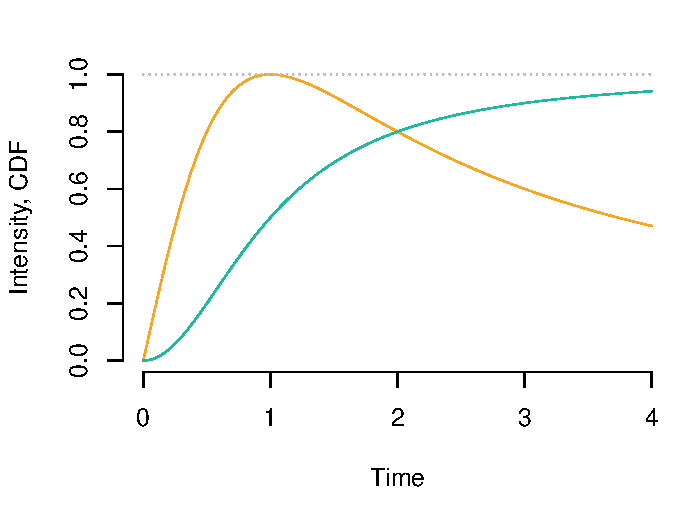
\includegraphics[width=\textwidth]{\FIGDIR/dwellDist01}
    \caption{$q(t) = \frac{2t}{t^2 + 1}$}
  \end{subfigure}
	\hfill
	\begin{subfigure}[b]{0.45\textwidth}
    \centering
		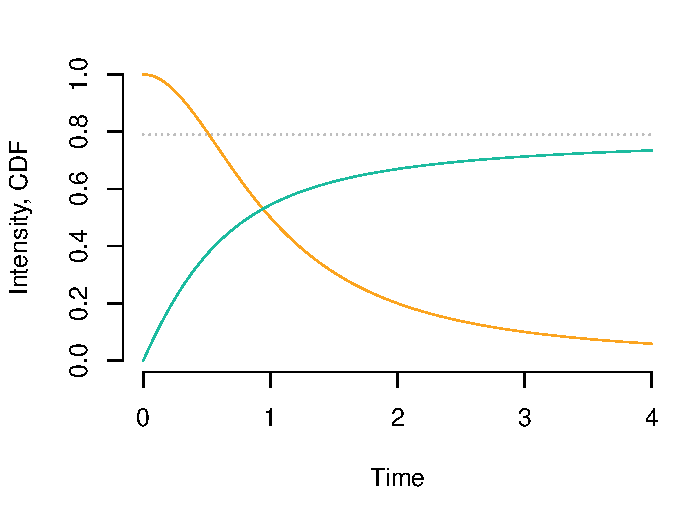
\includegraphics[width=\textwidth]{\FIGDIR/dwellDist02}
    \caption{$q(t) = \frac{1}{t^2 + 1}$}
  \end{subfigure}

	\begin{subfigure}[b]{0.45\textwidth}
    \centering
		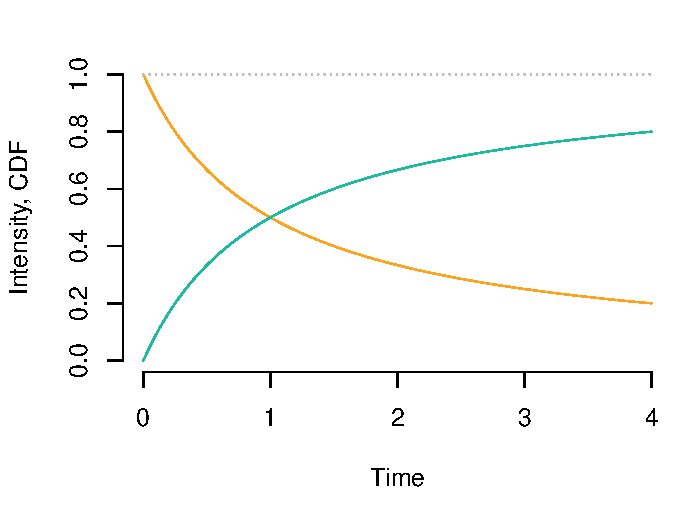
\includegraphics[width=\textwidth]{\FIGDIR/dwellDist03}
    \caption{$q(t) = \frac{1}{t + 1}$}
  \end{subfigure}
	\hfill
	\begin{subfigure}[b]{0.45\textwidth}
    \centering
		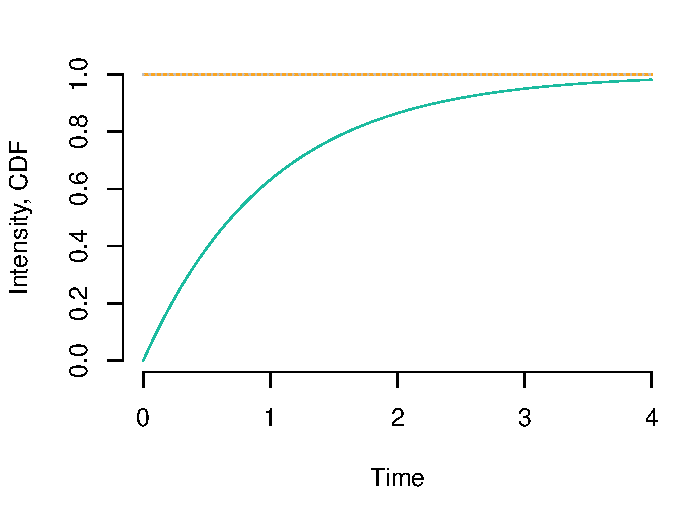
\includegraphics[width=\textwidth]{\FIGDIR/dwellDist04}
    \caption{$q(t) = 1$}
  \end{subfigure}

	\caption{Comparison of several transition rates (orange lines), their respective cumulative distribution functions of dwell time (blue lines), and limits of CDF (gray dashed lines. In the last plot we can see CDF of exponential distribution Exp(1).}
	\label{fig:dwellDist}
\end{figure}

\begin{proposition}
	\label{prop:transProb}
	Suppose that Markov process $\m{X}$ is at state $i$ up to time $t$ and at time $t$ leaves. Then it transitions into state $j$ with probability
	\[
		\pr [X_t = j \vert \lim_{s \to t^+} X_s = i, X_t \neq i ] = \frac{q_{ij}(t)}{q_{i}(t)}.
	\]
\end{proposition}

\begin{proof}
	Let \{s_k, k \in \N_0 \} be any increasing sequence with $s_k \to t$ as $k \to \infty$. Clearly the elements
	\[
		A_k = [ X_s = i, s \in [s_0, s_k], X_t \neq i ]
	\]
	are monotone as well with $A_1 \supset A_2 \supset ...$. Then we can write
	\[
		\pr [X_t = j \vert \lim_{s \to t^+} X_s = i, X_t \neq i ] = \lim_{k \to \infty} \pr [X_t = j \vert A_k].
	\]
	Because \X is Markov process it only depends on the state at the last known time and we have
	\[
		\pr [X_t = j \vert A_k] = \pr [X_t = j \vert X_{s_k}= i, X_t \neq i ] = \frac{p_{ij} (s_k, t)}{1-p_{ii} (s_k, t)}.
	\]
	After applying the limits we arrive to required.
\end{proof}

\begin{proposition}
	Let random variable $\tau_{s,i}$ be the first time process leaves state $i$ after time $s \geq 0$ and $X_s = i$, i.e. the random variable defined by \eqref{eq:tausi}. The process first transitions into state $j$ with probability
	\begin{equation}
		\label{eq:transProb}
		\pr [X_{\tau_{s,i}} = j \vert X_s = i ] = \E \left[ \frac{q_{ij}(\tau_{s,i})}{q_i(\tau_{s,i})} \right].
	\end{equation}
\end{proposition}

\begin{proof}
	Denote $F_{\tau}$ the cumulative distribution function of random variable $\tau_{s,i}$ and recall the support of $\tau_{s,i}$ is interval $(s, \infty)$. Then, by applying continuous Bayes' formula, we get
	\begin{multline*}
		\pr [X_{\tau_{s,i}} = j \vert X_s = i ] 
		= \int_s^\infty \pr [X_{\tau_{s,i}} = j \vert X_s = i, \tau_{s,i} = t] dF_{\tau} (t) \\
		= \int_s^\infty \pr [X_{t} = j \vert X_r = i, s \leq r < t] dF_{\tau} (t)
		= \int_s^\infty \frac{q_{ij}(t)}{q_{i}(t)} dF_{\tau} (t)
		= \E \left[ \frac{q_{ij}(\tau_{s,i})}{q_i(\tau_{s,i})} \right].
	\end{multline*}
\end{proof}

Note that the transition probability \eqref{eq:transProb} from previous proposition can be rewritten using the density of dwell time as
\[
	\E \left[ \frac{q_{ij}(\tau_{s,i})}{q_i(\tau_{s,i})} \right] =
	\int_0^\infty \exp \left(- \int_{s}^{s+x} q_i(t) dt \right) q_{ij}(s+x) dx.
\]

\begin{definition}
	\label{def:embedded}
	Let $\procX$ be a Markov process with transition times $T_1, T_2, ...$. Then we call a sequence of random variables
	\[
		\{ Y_k = X_{T_k}, k \in \N \}
	\]
	an \emph{embedded chain}.
\end{definition}

It is easy to find a contra-example to show that the embedded chain not necessarily has the Markov property. However, we are still able to derive its distribution.

\begin{corollary}
	Let Markov process $\procX$ enter the state $i$ at time $s$. Then the joint distribution of the dwell time and the new state has the density
	\[
		f_{s,i} (x, j) = \exp \left(- \int_{s}^{s+x} q_i(t) dt \right) q_{i,j}(s+x)
	\]
	with respect to product of Lebesgue measure on $(0, \infty)$ and counting measure on $S \setminus \{i\}$.
\end{corollary}

\begin{proof}
	The joint density is a product of marginal density of dwell time (Proposition~\ref{prop:dwellTime}) and conditional transition probability (Proposition~\ref{prop:transProb})
\end{proof}

	
	
	




%%%%%%%%%%%%%%%%%%%%%%%%%%%%%%%%%%%%%%%%%%%%%%%%%%%%%%%%%%%%%%%%%%%%%%%%%%%%%%%%%%%%%%%
%%%%%%%%%%%%%%%%%%%%%%%%%%%%%%%%%%%%%%%%%%%%%%%%%%%%%%%%%%%%%%%%%%%%%%%%%%%%%%%%%%%%%%%
\section{Separable Inhomogeneity}
\label{chap:separable}

In this section, we will study family of inhomogeneous Markov processes for which transition rates vary over time in the same manner for each transition between all pairs $i, j \in S$.

\begin{definition}
	\label{def:separable}
	Let $\procX$ be inhomogeneous Markov process with transition matrix $\m{Q} (t)$. If there exists a function $\lambda: \Rplus \to (0, \infty)$ and matrix $\m{\Gamma}$ such that
\[
	\m{Q}(t) = \lambda(t) \m{\Gamma}, \qquad \forall t \geq 0
\]
then we say that $\m{X}$ is Markov process with \emph{separable inhomogeneity}.

We will call $\lambda$ a \emph{separated inhomogeneity} and $\m{\Gamma}$ a \emph{constant rate matrix}.
\end{definition}

\begin{definition}
	\label{def:homoTrans}
	Suppose that $\procX$ is an inhomogeneous Markov process and $\m{Y} = \{Y_t, \, t \geq 0 \}$ is a homogeneous Markov process. We say that $\m{Y}$ is \emph{homogeneous transformation} of $\m{X}$ if there exists an increasing and differentiable function $\tau : \Rplus \to \Rplus$, $\tau (0) = 0$ such that $X_{\tau(t)} = Y_t$ a.s.
\end{definition}

Following theorem justifies the equivalency of previous definitions. The proof of the theorem is constructive and the reader can find a way how to calculate the time-transformation function $\tau$ and separated intensity function $\lambda$.

\begin{proposition}
	\label{prop:separable}
	Markov process $\procX$ has separable inhomogeneity if and only if there exists a homogeneous transformation of $\X$.
\end{proposition}

\begin{proof}
	Let $\X$ has separable inhomogeneity with notation from Definition~\ref{def:separable}. Define $\m{Y}$ as $Y_t = X_{\tau(t)}$, where $\tau(t) = \Lambda^{-1} (t)$. Because the function $\tau$ is increasing, the Markov property holds for the process $\m{Y}$ as well. The transition probabilities of $\Y$ are given by
	\begin{align*}
		p_{ij}^{(Y)} (t, t+h)
		=& \pr [ Y_{t+h} = j \vert Y_t = i ]
		= \pr [ X_{\tau (t+h)} = j \vert X_{\tau (t)} = i ] \\
		=& \lambda(\tau (t)) \gamma_{ij} \left( \Lambda^{-1} (t+h) - \Lambda^{-1} (t) \right) + o(h).
	\end{align*}
	The derivative of inverse function is given by
	\[
		\frac{\partial \Lambda^{-1} (t)}{\partial t} = \frac{1}{\lambda (\Lambda^{-1} (t))},
	\]
	which implies that the intensity of $\m{Y}$ is $q_{ij}^{(Y)} (t) = \gamma_{ij}$ and does not depend on time $t$.
	
	Suppose there exists a process $\m{Y}$ that is a homogeneous transformation of $\X$ with time-transformation function $\tau$ as in Definition~\ref{def:homoTrans} and the intensity matrix of $\m{Y}$ is $\bm{\Gamma}$. The transition probabilities of $\X$ are given by
		\begin{align*}
		p_{ij}^{(X)} (t, t+h)
		=& \pr [ X_{t+h} = j \vert X_t = i ]
		= \pr [ Y_{\tau^{-1} (t+h)} = j \vert Y_{\tau^{-1} (t)} = i ] \\
		=& \gamma_{ij} \left( \tau^{-1} (t+h) - \tau^{-1} (t) \right) + o(h).
	\end{align*}
	Therefore $\X$ has separated inhomogeneity with constant rate matrix $\bm{\Gamma}$ and function
	\[
		\lambda(t) = \frac{\partial \tau^{-1} (t)}{\partial t}.
	\]

\end{proof}

	
	




%%%%%%%%%%%%%%%%%%%%%%%%%%%%%%%%%%%%%%%%%%%%%%%%%%%%%%%%%%%%%%%%%%%%%%%%%%%%%%%%%%%%%%%
%%%%%%%%%%%%%%%%%%%%%%%%%%%%%%%%%%%%%%%%%%%%%%%%%%%%%%%%%%%%%%%%%%%%%%%%%%%%%%%%%%%%%%%
\section{Inhomogeneous Poisson Process}
\label{chap:poisson}

Poisson process is widely used as a counting process for number of events that occur independently over a time interval. In practice, sometimes we face problems that violate the assumptions of homogeneity of the Poisson process. In this section we introduce processes that generalize the definition of Poisson process. Let us begin with definition of inhomogeneous Poisson process.

\begin{definition}
	\label{def:inhomogeneousPoisson}
	Suppose that $N = \{N_t, t \geq 0\}$ is a counting process with values in $\N_0$ and $\lambda : \Rplus \to \Rplus$ be a real function. We call $N$ an \emph{inhomogeneous Poisson process} if it follows
	\begin{enumerate}[i)]
		\item $N_0 = 0$ a.s.;
		\item Increments of $N$ are independent;
		\item $\pr [ N_{t+h} = i+1 \vert N_t = i ] = \lambda(t) h + o(h)$;
		\item $\pr [ N_{t+h} > i+1 \vert N_t = i ] = o(h)$.
	\end{enumerate}
\end{definition}

Clearly, if $\lambda$ is constant, non-zero function then $N$ is homogeneous Poisson process. Inhomogeneous Poisson process is a special case of Markov process with separable inhomogeneity with transition rate matrix
\[
	\m{Q}(t) = \begin{pmatrix}
			-\lambda (t) & \lambda (t) & 0 & \cdots \\
			0 & -\lambda (t) & \lambda (t) &  \\
			\vdots & & \ddots & \ddots
\end{pmatrix} = \lambda (t) \begin{pmatrix}
			-1 & 1 & 0 & \cdots \\
			0 & -1 & 1 &  \\
			\vdots & & \ddots & \ddots
\end{pmatrix}.
\]

The distribution of Poisson process is again Poisson, i.e.
\[
	N_t \sim Poi (\Lambda(t)), \text{ where } \Lambda(t) = \int_0^t \lambda(t) dt.
\]
The reader can find a proof for example in \cite{Lewis79}. Another way to show this is to use the fact that the inhomogeneous Poisson process is also an inhomogeneous Markov process with separable inhomogeneity. Then there exists by \nameref{prop:separable} a homogeneous transformation with unit intensity and transformation function $\tau (t) = \Lambda^{-1} (t)$. This can be used to simulate an inhomogeneous Poisson process on time interval $[0, T]$.

\begin{algorithm}[Simulating Poisson process]\
	\label{algo:simulPoisson}
	\begin{enumerate}
		\item Simulate number of transitions $N \sim Poi (\Lambda(T))$.
		\item Simulate independent random variables $R_i \sim Exp(1)$ for $i = 1, ..., N+1$.
		\item Calculate ordered transition times of the homogeneous transformation on interval $[0,1]$
			\[
				S_k = \frac{\sum_{i=1}^{k} R_i}{\sum_{i=1}^{N+1} R_i}, \qquad k = 1, ..., N.
			\]
		\item Transform to transition times of the inhomogeneous Poisson process
			\[
				T_k = \Lambda^{-1} (S_k \times \Lambda(T)), \qquad k = 1, ..., N,
			\]
		\item Return the transition times $T_1, ..., T_N$.
	\end{enumerate}
\end{algorithm}



Denote by $T_1, T_2, ...$ the increasing sequence of (random) jump times of inhomogeneous Poisson process. Their distributions are given by Proposition \ref{prop:dwellTime}. Let $Z_1, Z_2, ...$ be a sequence of independent random variables with distribution measures $\mu_{T_i}$. Then we can define random process by
\[
	M_t = \sum_{i=1}^{\infty} Z_i \times \mathbb{I} [t \geq T_i].
\]
Let us call this process an \emph{inhomogeneous compound Poisson process}. In following Proposition we show the property of such process if the distributions of $Z_i$ are Bernoulli.

\begin{proposition}
	\label{prop:compoundPoisson}
	Let $N = \{N_t, t \geq 0\}$ be an inhomogeneous Poisson process with intensity $\lambda(t)$ and jump times $T_1, T_2, ...$. Let $\pi: \Rplus \to (0,1)$ be a right-continuous function and $Z_i \sim Alt(\pi(T_i))$. Then the family of random variables
	\[
		M_t = \sum_{i=1}^{\infty} Z_i \times \mathbb{I} [t \geq T_i].
	\]
	is an inhomogeneous Poisson process with intensity $\lambda(t) \pi(t)$.
\end{proposition}

\begin{proof}
	Since $M$ is non-negative process and $M_t \leq N_t$ a.s. for any $t \geq 0$, then also $M_0 = 0$ a.s. The increments of $N$ are independent by definition and also the values of $Z_i$ are mutually independent. The increments of $M$ are also independent.
	
	Because the function $\pi$ is right continuous, one can write $\pi(t+h) = \pi(t) + o(h)$. The probability of jump in a small interval is bounded by
	\begin{align*}
		\pr [ M_{t+h} = j+1 \vert M_t = j ]
		&\geq \pr [ N_{t+h} = i+1 \vert N_t = i ] \times (\pi(t) + o(h)) \\
		&= (\lambda(t) h + o(h)) \times (\pi(t) + o(h)) = \lambda(t)\pi(t) h + o(h)\\
	\end{align*}
	and
	\begin{align*}
		\pr [ M_{t+h} = j+1 \vert M_t = j ]
		&\leq \lambda(t)\pi(t) h + o(h) + \pr [ N_{t+h} > i+1 \vert N_t = i ] \\
		&= \lambda(t)\pi(t) h + o(h),
	\end{align*}
	Which implies that the probability is equal to both the boundaries. Also
	\[
		\pr [ M_{t+h} > j+1 \vert M_t = j ] \leq \pr [ N_{t+h} > i+1 \vert N_t = i ]
	\]
	implies point \emph{iv} in Definition~\ref{def:inhomogeneousPoisson}.
\end{proof}
	\chapter{Estimating Transition Intensity}
	\label{chap:statistics}

In this chapter, we build several parametric models for intensity functions of inhomogeneous Markov process. For each of the models we propose a method for estimating the parameter using maximum likelihood. The theory of maximum likelihood estimates (MLE) is not described in this thesis. The reader can find general results for example in~\cite{Andel11}, Chapter~7.6. We try to keep the notation close to the notation at said book.

We will estimate the parameter using embedded Markov chain and dwell times of multiple observations of Markov process on the same time interval. Let $\mathbf{X}^1, \dots, \mathbf{X}^n$ be a random sample from distribution of inhomogeneous Markov process with state space $S$, intensity $\m{Q} (t; \bm{\theta}_X)$, and initial probability $\m{p} (\bm{\theta}_X)$, where $\bm{\theta}_X \in \R^H$ is the unknown parameter. Denote by $K^{\nu}$ the number of jumps of process $\mathbf{X}^{\nu}$, by $T^{\nu}_1, ... , T^{\nu}_{K^{\nu}}$ the times of jumps and by $Y^{\nu}_0, ... , Y^{\nu}_{K^{\nu}}$ the embedded Markov chain.

The likelihood function is of form
\begin{multline}
	L_n (\bm{\theta}; \mathbf{X}^1, \dots, \mathbf{X}^n) \\
	=
	\prod_{\nu=1}^n \Biggl[ p_{Y_0} (\mathbf{ \bm{\theta} })
	\prod_{k=1}^{K^{\nu}} \left[ f_{T_{k-1}^{\nu}, Y_{k-1}^{\nu}} (T_k^{\nu} - T_{k-1}^{\nu}; \mathbf{ \bm{\theta} }) \: \frac{q_{ij} (T_k^{\nu}; \mathbf{ \bm{\theta} })}{q_{i} (T_k^{\nu}; \mathbf{ \bm{\theta} })} \right]
	\\ 
	\times \left( 1-F_{T_{K^{\nu}}^{\nu},Y_{K^{\nu}}^{\nu}} (T-T_{K^{\nu}}^{\nu}; \mathbf{ \bm{\theta} }) \right) \Biggr],
	\label{eq:generalLik}
\end{multline}
where
\[
	F_{s,i} (x; \bm{\theta}) = 1 - \exp \left(- \int_{s}^{s+x} q_i(t; \bm{\theta}) dt \right)
\]
is the cumulative distribution function of the dwell time given that the process transitions at time $s$ into state $i$ and
\[
	f_{s,i} (x; \bm{\theta}) = \exp \left(- \int_{s}^{s+x} q_i(t; \bm{\theta}) dt \right) q_i(s+x; \bm{\theta})
\]
is the respective probability density function.

Let use denote the likelihood function by $L_n (\bm{\theta})$ and exclude the observed data $\mathbf{X}^1, \dots, \mathbf{X}^n$ from the notation. Further we use standard notation $\ell_n (\bm{\theta}) = \log(L_n (\bm{\theta}))$ for log-likelihood, $\m{U}_n (\bm{\theta}) = \partial \ell_n (\bm{\theta}) / \partial \bm{\theta}$ for the score function, $\m{I}_n (\bm{\theta}) = -1/n \times \partial \m{U}_n (\bm{\theta}) / \partial \bm{\theta}$ for the observed information matrix, and $\m{I} (\bm{\theta}) = \E [\m{I}_n (\bm{\theta})]$ for the Fisher information matrix.

The true vector parameter $\bm{\theta}_X$ is estimated by parameter $\hat{\bm{\theta}}_n$ that maximizes the likelihood function. In most cases, that is equivalent to solving the system of equations $\m{U}_n (\bm{\theta}) = \m{0}$.

In general case, one cannot calculate $\hat{\bm{\theta}}_n$ directly by solving the system of equations $\m{U}_n (\bm{\theta}) = \m{0}$. The MLE must be calculated by some numerical method. Here, we explain Newton-Raphson method. The method is iterative and updates the vector parameter at each iteration. Denote by $\bm{\theta}^{(r)}$ the $r$-th iteration of the algorithm. The $(r+1)$-th iteration is given by
\[
	\bm{\theta}^{(r+1)} = \bm{\theta}^{(r)} + \left[ n \m{I}_n (\bm{\theta}^{(r)}) \right]^{-1} \m{U}_n (\bm{\theta}^{(r)}).
\]
The algorithm is iterated until the value of $\m{U}_n (\bm{\theta}^{(r)})$ is sufficiently close to $\m{0}$. If the starting value $\bm{\theta}^{(0)$ is well chosen, the algorithm converges to the solution, i.e. $\bm{\theta}^{(r)} \to \hat{\bm{\theta}}_n$ as $r \to \infty$.


%%%%%%%%%%%%%%%%%%%%%%%%%%%%%%%%%%%%%%%%%%%%%%%%%%%%%%%%%%%%%%%%%%%%%%%%%%%%%%%%%%%%%%%
%%%%%%%%%%%%%%%%%%%%%%%%%%%%%%%%%%%%%%%%%%%%%%%%%%%%%%%%%%%%%%%%%%%%%%%%%%%%%%%%%%%%%%%
\section{Homogeneous Markov Process}
	\label{chap:statHomo}

The simplest Markov process is the homogeneous case. The intensity is constant in time and depends only on the unknow parameter $\bm{\theta}$, i.e. for each $i,j \in S$ we can write
\begin{align*}
	q_{ij} (t; \mathbf{ \bm{\theta} }) &= q_{ij} (\mathbf{ \bm{\theta} }), \\
	q_{i} (t; \mathbf{ \bm{\theta} }) &= q_{i} (\mathbf{ \bm{\theta} }).
\end{align*}
Also the cumulative distribution function and density can be simplified as
\begin{align*}
	F_{t,i} (x; \mathbf{ \bm{\theta} }) &= 1 - \e^{-x q_i(\mathbf{ \bm{\theta} })}, \\
	f_{t,i} (x; \mathbf{ \bm{\theta} }) &= q_i(\mathbf{ \bm{\theta} }) \e^{-x q_i(\mathbf{ \bm{\theta} })}.
\end{align*}
Finally, the log-likelihood function is
\begin{multline*}
	\ell_n (\mathbf{ \bm{\theta} }; X^1, \dots, X^n) \\
	= \sum_{\nu=1}^n \Biggl[ \log( p_{Y_0^{\nu}} (\bm{\theta})) +
	\sum_{k=1}^{K^{\nu}} \bigg[ \log( q\indexij (\bm{\theta}) )
	- q\indexi (\bm{\theta}) (T_k^{\nu} - T_{k-1}^{\nu}) \bigg] 
	- \\
	- q_{Y_{K^{\nu}}^{\nu}} (\mathbf{\bm{\theta}}) (T-T_{K^{\nu}}^{\nu}) \right) \Biggr].
\end{multline*}

This setup is still to general to derive any result that could be applicable to every parametrization of the intensity. Instead of that, we derive the properties of MLE for one special case. This process and its properties are taken from \cite{PraskovaLachout12}, Chapter 3.5.

\begin{example}[Linear Growth Process]
	The process is defined on state space $S = \N$ with inception at point $i=1$ and intensities
	\[
		q_{ij} (\theta) = \begin{cases}
			-i \theta \qquad & \text{if } j=i \\
			i \theta \qquad & \text{if } j=i+1 \\
			0 \qquad & \text{else,}
		\end{cases}
	\]
	where $\theta > 0$ is an unknown parameter (one-dimensional).
	
	The distribution of the process at fixed time is given by (see the referred book for proof)
	\[
		p_{1j} (0,t) = \e^{-j t \theta} (\e^{t \theta} - 1)^{j-1}.
	\]
	That implies that the expected value is
	\begin{equation}
		\label{eq:LGPmean}
		\E [X_t] = \sum_{j=1}^{\infty} j \e^{-j t \theta} (\e^{t \theta} - 1)^{j-1} = \e^{t \theta}.
	\end{equation*}
	
	Because the process is straightforward and for each state $i \in S$ there exists exactly one state $j \in S$ for which the process can transition from $i$ to $j$, we know that $Y_k = k+1$. With that, we can write	
	\begin{align*}
		q_{Y_{k-1},Y_{k}} (\theta) &= q_{k,k+1} (\theta) = k \theta \\
		q_{Y_{k-1}} (\theta) &= q_{k} (\theta) = k \theta \\
		p_{Y_0} &= p_1 = 1
	\end{align*}
	
	Suppose we observe a random sample of size $n$ over time interval $[0,T]$. The log-likelihood function is	
	\[
		\ell_n (\theta)
		= \sum_{\nu=1}^n \Biggl[ \sum_{k=1}^{K^{\nu}} \bigg[ \log( k \theta) - k \theta (T_k^{\nu} - T_{k-1}^{\nu}) \bigg] 
		- (K^{\nu}+1) \theta (T-T_{K^{\nu}}^{\nu}) \Biggr],
	\]
	the score function is
	\[
		U_n (\theta)
		= \sum_{\nu=1}^n \Biggl[ K^{\nu} \frac{1}{\theta} - \sum_{k=1}^{K^{\nu}} k (T_k^{\nu} - T_{k-1}^{\nu}) 
		+ (K^{\nu}+1) (T-T_{K^{\nu}}^{\nu}) \Biggr],
	\]
	and the observed information matrix is
	\[
		I_n (\theta)
		= \frac{1}{n} \sum_{\nu=1}^n K^{\nu} \frac{1}{\theta^2}
		= \overline{K} \frac{1}{\theta^2}
	\]
	where $\overline{K} = \frac{1}{n} \sum_{\nu=1}^n K^{\nu}$ denotes the mean number of jumps.
	
	Solving the equation $U_n (\theta) = 0$ one get the MLE
	\[
		\hat{\theta}_n = \frac
			{\sum_{\nu=1}^n K^{\nu}}
			{\sum_{\nu=1}^n \Bigr[\sum_{k=1}^{K^{\nu}} k (T_k^{\nu} - T_{k-1}^{\nu}) + (K^{\nu}+1) (T-T_{K^{\nu}}^{\nu}) \Bigl]}
	\]
	
	Given the fact that $K^{\nu} = X_T^{\nu} - 1$ and (\ref{eq:LGPmean}) one can calculate the Fisher information matrix
	\[
		I (\theta)
		= \E [I_n (\theta)]
		= \frac{\e^{T \theta} - 1}{\theta^2}.
	\]
	The asymptotic distribution of the estimate is
	\[
		\sqrt{n} (\hat{\theta}_n - \theta_X) \gotod N \left( 0, \frac{\theta_X^2}{\e^{T \theta_X} - 1} \right)
		\text{ as } n \to \infty,
	\]
where $\theta_X$ denotes the true parameter.
	
	\demo
\end{example}

At the end of this section, let us state a proposition about estimation of full model. The result is straightforward and intuitive and the proposition is left without a proof.

\begin{proposition}
	Let $\m{X}^1, ..., \m{X}^n$ be a random sample from homogeneous Markov process with transition rate $\m{Q} = (q_{ij})_{i,j \in S}$ and initial probability vector $\m{p} = (p_i)_{i \in S}$. Denote by $N_{ij}$ total number of transitions from state $i$ to state $j$, by $M_i$ number of processes that initiates at state $i$, and by $T_i$ total time spent in state $i$. If $T_i > 0$, the MLE estimator of transition rates and initial probabilities are
	\begin{align*}
		\widehat{q_{ij}} = \frac{N_{ij}}{T_i}, \qquad
		\widehat{p_i} = \frac{M_i}{n}.
	\end{align*}
	If $T_i = 0$, the result for initial probabilities holds and any estimate $\widehat{q_{ij}} \geq 0$ maximizes the (log-)likelihood.
	\label{prop:generalMC}
\end{proposition}

Note that MLE estimators from Proposition~\ref{prop:generalMC} does not fulfill regularity conditions and not all results valid from MLE theory hold.
%Further, it is clear that the MLE of initial probabilities hold when initial probabilities and transition rates are independent, i.e. we are able to separate the vector parameter (after reordering) $\bm{\theta} = (\bm{\theta_1}, \bm{\theta_2})$ such that $\m{p} (\bm{\theta}) = \m{p} (\bm{\theta_1})$ and $\m{Q} (\bm{\theta}) = \m{Q} (\bm{\theta_2})$. Because of that, we will assume in following that the vector of initial probabilities is known.




%%%%%%%%%%%%%%%%%%%%%%%%%%%%%%%%%%%%%%%%%%%%%%%%%%%%%%%%%%%%%%%%%%%%%%%%%%%%%%%%%%%%%%%
%%%%%%%%%%%%%%%%%%%%%%%%%%%%%%%%%%%%%%%%%%%%%%%%%%%%%%%%%%%%%%%%%%%%%%%%%%%%%%%%%%%%%%%
\section{Separated Inhomogeneity}
	\label{chap:statSeparInhom}
	
	From this chapter on, we assume that the distribution of initial probability $\m{p}$ is known and does not depend on the unknown parameter $\bm{\theta}$. In most of the examples we show in this thesis, the initial distribution is concentrated in single state space (either $p_0 = 1$ or $p_1 = 1$).

Assume that $\m{X}$ is Markov process process with separable inhomogeneity, i.e. its transition rate matrix is
\[
	\m{Q}(t) = \lambda(t) \m{\Gamma}, \qquad \forall t \geq 0.
\]
Let us further assume that the constant rate matrix $\m{\Gamma} = \{\gamma_{ij}, i,j \in S \}$ is known and separated inhomogeneity $\lambda$ follows a log-linear model
\begin{equation}
	\label{eq:logLinearIntensity}
	\lambda (t; \bm{\beta}) = \exp \left( \sum_{h=0}^{H} \beta_h \varphi_h (t) \right), \qquad \forall t \geq 0,
\end{equation}
where $\varphi_h: \Rplus \to \R$ is given continuous function for $h = 0, ..., H$ and $\bm{\beta} = (\beta_0, ..., \beta_H)$ is vector of unknown parameters. Usually, we take $\varphi_0 = 1$ and call $\beta_0$ an intercept. The derivative of separated inhomogeneity with respect to parameter vector is
\[
	\frac{\partial \lambda (t; \bm{\beta})}{\partial \bm{\beta}} = \lambda (t; \bm{\beta}) \T{(\varphi_0 (t), ..., \varphi_H (t))} \equiv \lambda (t; \bm{\beta}) \bm{\varphi} (t).
\]

We can adjust the likelihood function~\eqref{eq:generalLik} for this particular case and calculate log-likelihood function
\begin{multline*}
	\ell_n (\bm{\beta})
	= \sum_{\nu=1}^n \Biggl[ \log( p_{Y_0^{\nu}}) +
	\sum_{k=1}^{K^{\nu}} \bigg[ \log(\gamma\indexij) + \T{\bm{\beta}} \bm{\varphi} (T_k^{\nu}) - \\
	- \gamma\indexi \int_{T_{k-1}^{\nu}}^{T_k^{\nu}} \lambda(t; \bm{\beta}) dt \bigg] -
	\gamma_{Y_{K^{\nu}}^{\nu}} \int_{T_{K^{\nu}}^{\nu}}^{T} \lambda(t; \bm{\beta}) dt \Biggr],
\end{multline*}
the score statistic
\begin{multline*}
	\m{U}_n (\bm{\beta})
	= \sum_{\nu=1}^n \Biggl[ \sum_{k=1}^{K^{\nu}} \bigg[ \bm{\varphi} (T_k^{\nu}) -
	\gamma\indexi \int_{T_{k-1}^{\nu}}^{T_k^{\nu}} \lambda(t; \bm{\beta}) \bm{\varphi} (t) dt \bigg] - \\
	- \gamma_{Y_{K^{\nu}}^{\nu}} \int_{T_{K^{\nu}}^{\nu}}^{T} \lambda(t; \bm{\beta}) \bm{\varphi} (t) dt \Biggr],
\end{multline*}
	and the observed information matrix
\begin{multline*}
	\m{I}_n (\bm{\beta})
	= \frac{1}{n} \sum_{\nu=1}^n \Biggl[ \sum_{k=1}^{K^{\nu}}
	\gamma\indexi \int_{T_{k-1}^{\nu}}^{T_k^{\nu}} \lambda(t; \bm{\beta}) \bm{\Omega} (t) dt
	+ \gamma_{Y_{K^{\nu}}^{\nu}} \int_{T_{K^{\nu}}^{\nu}}^{T} \lambda(t; \bm{\beta}) \bm{\Omega} (t) dt \Biggr],
\end{multline*}
where	$\bm{\Omega} (t) = \bm{\varphi} (t) \T{(\bm{\varphi} (t))}$ for all $t \geq 0$.

It is not possible to solve the system of equations $\m{U}_n (\bm{\beta}) = \bm{0}$ directly and one needs to use the Newton-Raphson iterative method to find the MLE $\hat{\bm{\beta}}_n$.

\begin{example}[Testing homogeneity of Poisson Process]
	While testing homogeneity of Poisson process, we are interested in test of null hypothesis $H_0$ against alternative hypothesis $H_1$, where
	\begin{align*}
		H_0 &: \forall s,t \in [0,T] : \lambda(s) = \lambda(t), \\
		H_1 &: \exists s,t \in [0,T] : \lambda(s) \neq \lambda(t).
	\end{align*}
	This hypothesis is hard to test. Instead of that, we will provide a weaker test in model~(\ref{eq:logLinearIntensity})
		\begin{align*}
			H_0 &: \beta_1 = ... = \beta_H = 0 \\
			H_1 &: \exists h \in \{1, ..., H\} : \beta_h \neq 0.
	\end{align*}
	Denote the vector parameter under null hypothesis by $\bm{\beta}_0 = (\beta_{0,0}, 0, ..., 0)^{\top}$, where $\beta_{0,0} \in \R$ is nuisance parameter. The intensity under null hypothesis is $\lambda(t, \bm{\beta}_0) = \e^{\beta_{0,0}}$. The MLE of $\beta_{0,0}$ under null hypothesis is $\tilde{\beta}_{0,n} = \log (\frac{1}{n} \sum_{\nu = 1}^n X_T^{\nu})$.
	
	We already know (from Chapter~\ref{chap:poisson}) that inhomogeneous Poisson process is inhomogeneous Markov process with unit constant rate from state $i$ to $i+1$, where $i \in \N_0$, i.e. $\gamma_{i} = \gamma_{i,i+1} = 1$ for each $i \in S$. 
	
	The score statistic is simplified into
	\[
		\m{U}_n (\bm{\beta})
		= \sum_{\nu=1}^n \sum_{k=1}^{K^{\nu}} \bm{\varphi} (T_k^{\nu})
		- n\int_{0}^{T} \lambda(t; \bm{\beta}) \bm{\varphi} (t) dt.
	\]
		The observed information matrix does not depend on the data and, therefore, is equal to Fisher information matrix, i.e. 
	\[
		\m{I}_n (\bm{\beta}) =
		\int_{0}^{T} \lambda(t; \bm{\beta}) \bm{\Omega} (t) dt = 
		\m{I} (\bm{\beta}).
	\]
	
		Without loss of generality assume $T = 1$. Suppose the model is given by $\varphi_h (t) = t^h$. Then the matrix $\bm{\Omega} (t)$ at position $i,j$ is equal to $t^{i+j-2}$ and the respective position of Fisher information matrix $\m{I} (\bm{\beta}_0)$ is (if the null hypothesis holds)
		\[
			\int_0^1 \e^{\beta_{0,0}} t^{i+j-2} dt = \frac{\e^{\beta_{0,0}}}{i+j-1}.
		\]
		Since $\tilde{\bm{\beta}}_n = (\tilde{\beta}_{0,n}, 0, ..., 0)^{\top}$ is consistent estimate of $\bm{\beta}_0$ under null hypothesis, also the matrix
		\[
			\m{I} (\tilde{\bm{\beta}}_n) = \left\{ \frac{\sum_{\nu = 1}^n X_T^{\nu}}{n (i+j-1)}; i,j = 1, ..., H+1 \right\}
		\]
		is consistent estimate of $\m{I} (\bm{\beta}_0)$. The Rao score statistic is		
		\[
			R_n = \frac{1}{\sum_{\nu = 1}^n X_T^{\nu}} \m{U}_{-1,n} (\tilde{\bm{\beta}}_n) ^{\top} \left[ [ \mathcal{H}_{H+1} ]^{-1} \right]_{-1,-1} \m{U}_{-1,n} (\tilde{\bm{\beta}}_n),
		\]
		where $\m{U}_{-1,n} (\tilde{\bm{\beta}}_n)$ is the score function at point $\tilde{\bm{\beta}}_n$ where the first element is excluded and $\mathcal{H}_k$ is the $k \times k$ Hilbert matrix. By notation $A_{-i,-j}$ we indicate the matrix $A$ without $i$-th row and $j$-th column excluded. 
		The statistic has (under null hypothesis) $\chi^2$ distribution with $H$ degrees of freedom so one can reject the  null hypothesis if $R_n \geq \chi_H^2(1-\alpha)$.
		
		Note that we are able to calculate the Rao score statistic without calculating the MLE of $\bm{\beta}$ (without assumption that the null hypothesis holds).
		
	\demo
\end{example}




%%%%%%%%%%%%%%%%%%%%%%%%%%%%%%%%%%%%%%%%%%%%%%%%%%%%%%%%%%%%%%%%%%%%%%%%%%%%%%%%%%%%%%%
%%%%%%%%%%%%%%%%%%%%%%%%%%%%%%%%%%%%%%%%%%%%%%%%%%%%%%%%%%%%%%%%%%%%%%%%%%%%%%%%%%%%%%%
\section{Constant Rate Matrix}

In this chapter we follow notation from Chapter~\ref{chap:separable}. Suppose that the separated inhomogeneity function $\lambda$ is known and we are interested in estimating the constant rate matrix $\bm{\Gamma}$. We suppose that the matrix depends on unknown vector parameter $\bm{\theta}$. We denote the matrix by $\bm{\Gamma} (\bm{\theta})$. By Proposition \ref{prop:separable}, we are able to find a homogeneous transformation of the process $\m{X}$. Then, we can use this homogeneous transformation and results from Chapter~\ref{chap:statSeparInhom} to estimate the parameter $\bm{\theta}$.

If also the separated inhomogeneity were unknown, we cannot find the homogeneous transformation $X_{\tau(t)}$ and we need to estimate both the constant rate matrix and the separated inhomogeneity function. Suppose that the vector parameter is divided into $(\bm{\beta}^{\top}, \bm{\theta}^{\top})^{\top}$, where $\bm{\beta} \in \R^{H_1}$, $\bm{\theta} \in \R^{H_2}$, and $H_1 + H_2 = H$. Further suppose that function $\lambda = \lambda (\bm{\beta})$ follows log-linear model similar to Chapter~\ref{chap:statSeparInhom} and matrix $\bm{\Gamma} = \bm{\Gamma} (\bm{\theta})$ has similar parametrization as in Chapter~\ref{chap:statHomo}.

Note that we do not need to keep the intercept in the log-linear term for separated inhomogeneity function in most of reliable models. If for each $\bm{\theta} \in \Theta$ and $c > 0$ there exists $\bm{\theta}^{'} \in \Theta$ such that $\bm{\Gamma} (\bm{\theta}^{'}) = c \bm{\Gamma} ( \bm{\theta} )$, then it is easier to set $c = \e^{\beta_0} = 1$, i.e. the intercept $\beta_0 = 0$ needs not be included in the model.

The log-likelihood function
\begin{multline*}
	\ell_n (\bm{\beta}, \bm{\theta})
	= \sum_{\nu=1}^n \Biggl[ \log( p_{Y_0^{\nu}}) +
	\sum_{k=1}^{K^{\nu}} \bigg[ \log(\gamma\indexij (\bm{\theta})) + \T{\bm{\beta}} \bm{\varphi} (T_k^{\nu}) - \\
	- \gamma\indexi (\bm{\theta}) \int_{T_{k-1}^{\nu}}^{T_k^{\nu}} \lambda(t; \bm{\beta}) dt \bigg] -
	\gamma_{Y_{K^{\nu}}^{\nu}} (\bm{\theta}) \int_{T_{K^{\nu}}^{\nu}}^{T} \lambda(t; \bm{\beta}) dt \Biggr]
\end{multline*}
is again hard to work with without any assumption about the constant intensity rate $\bm{\Gamma} (\bm{\theta})$. Instead of deriving other statistics in general, we show one example of such model.

\begin{example}[Independent queuing systems]
	Suppose that there exist $H_2$ independent queuing systems for which the arrivals follow inhomogeneous processes. Further suppose that the queuing systems are mutually independent and the intensities of individual systems differs only in scale. Denote by $\lambda_h (t; \bm{\beta})$ the intensity of $h$-th system at time $t$ for $h = 1, ..., H_2$. Then the ratio $\lambda_h (t; \bm{\beta}) / \lambda_h (s; \bm{\beta})$ does not depend on the system $h$ for any $s,t \geq 0$ such that $\lambda_h (s; \bm{\beta}) > 0$. One reliable model for intensities could be
	\begin{equation*}
		\lambda_h (t; \bm{\beta}, \bm{\theta}) = \theta_h \exp \left( \sum_{h=1}^{H} \beta_h \varphi_h (t) \right), \qquad \forall t \geq 0, h=1,...,H_2.
	\end{equation*}
	
	Denote by $(i,j) \sim h$ the fact that that the transition from $i$ to $j$ is equivalent to one arrival in system $h$. Now, we can write the constant intensities as
	\[
		\gamma_{i,j} (\bm{\theta})= \sum_{h=1}^{H_2} \theta_h \mathbb{I} [(i,j) \sim h]
	\]
	and their derivations are $\partial \gamma_{i,j} (\bm{\theta}) / \partial \theta_h = \mathbb{I} [(i,j) \sim h]$. For each state $i \in S$ and system $h = 1, ..., H_2$ there exist exactly one state $j \in S$ such that $(i,j) \sim h$. Therefore, the total constant intensities are $\gamma_{i} (\bm{\theta})= \sum_{h=1}^{H_2} \theta_h \equiv s(\bm{\theta})$ for all $i \in S$.
	
	The first and the second derivatives of log-likelihood function with respect to vector parameters $\bm{\beta}$ and $\bm{\theta}$ are
	\begin{align*}
		\frac{\partial \ell_n (\bm{\beta}, \bm{\theta})}{\partial \bm{\beta}} &=
		\sum_{\nu=1}^n \sum_{k=1}^{K^{\nu}} \bm{\varphi} (T_k^{\nu}) 
		- n s(\bm{\theta}) \int_{T_{K^{\nu}}^{\nu}}^{T} \lambda(t; \bm{\beta}) \bm{\varphi} (t) dt,
		\\
				\frac{\partial \ell_n (\bm{\beta}, \bm{\theta})}{\partial \theta_h}
		&= \frac{1}{\theta_h} \sum_{\nu=1}^n
		\sum_{k=1}^{K^{\nu}} \mathbb{I} [(Y_{k-1}^{\nu}, Y_{k}^{\nu}) \sim h] -
		 n \int_{0}^{T} \lambda(t; \bm{\beta}) dt,
		\\
		\frac{\partial^2 \ell_n (\bm{\beta}, \bm{\theta})}{\partial \bm{\beta} \partial \bm{\beta}^{\top}}
		&= - n s(\bm{\theta}) \int_{0}^{T} \lambda(t; \bm{\beta}) \bm{\Omega} (t) dt.
		\\
		\frac{\partial^2 \ell_n (\bm{\beta}, \bm{\theta})}{\partial \bm{\beta} \partial \theta_h}
		&= - n \int_{0}^{T} \lambda(t; \bm{\beta}) \bm{\varphi} (t) dt,
		\\
		\frac{\partial^2 \ell_n (\bm{\beta}, \bm{\theta})}{\partial \theta_{h_1} \partial \theta_{h_2}}
		&= \frac{-1}{\theta_h_1^2} \sum_{\nu=1}^n
		\sum_{k=1}^{K^{\nu}} \mathbb{I} [(Y_{k-1}^{\nu}, Y_{k}^{\nu}) \sim h_1]
			\times \mathbb{I} [h_1 = h_2],
	\end{align*}
	
	Denote by $N_{n,h} = \sum_{\nu=1}^n \sum_{k=1}^{K^{\nu}} \mathbb{I} [(Y_{k-1}^{\nu}, Y_{k}^{\nu}) \sim h]$ the total number of arrivals in all observations of system $h$. Then we have the score function	
	\[
		\m{U}_n (\bm{\beta}, \bm{\theta}) = 
			\left(
			\begin{array}{c}
				\sum_{\nu=1}^n \sum_{k=1}^{K^{\nu}} \bm{\varphi} (T_k^{\nu})
				- n s(\bm{\theta}) \int_{T_{K^{\nu}}^{\nu}}^{T} \lambda(t; \bm{\beta}) \bm{\varphi} (t) dt
				\\
				\displaystyle{\frac{N_{n,1}}{\theta_1}} \sum_{\nu=1}^n -
				n \int_{0}^{T} \lambda(t; \bm{\beta}) dt
				\\
				\vdots
				\\
				\displaystyle{\frac{N_{n,H_2}}{\theta_{H_2}}} \sum_{\nu=1}^n -
				n \int_{0}^{T} \lambda(t; \bm{\beta}) dt
			\end{array}
			\right)
	\]
and the observed information matrix
	\[
		\m{I}_n (\bm{\beta}, \bm{\theta}) = 
			\left(
			\begin{array}{cc}
				s(\bm{\theta}) \int_{0}^{T} \lambda(t; \bm{\beta}) \bm{\Omega} (t) dt & \m{D}_{\bm{\theta}, \bm{\beta}}^{\top} \\
				\m{D}_{\bm{\theta}, \bm{\beta}}						                    & \m{D}_{\bm{\theta}, \bm{\theta}}
			\end{array}
			\right),
	\]
	where
	\[
		\m{D}_{\bm{\theta}, \bm{\beta}} = 
			\left(
			\begin{array}{c}
				\int_{0}^{T} \lambda(t; \bm{\beta}) \bm{\varphi} (t)^{\top} dt \\
				\vdots \\
				\int_{0}^{T} \lambda(t; \bm{\beta}) \bm{\varphi} (t)^{\top} dt
			\end{array}
			\right),
		\qquad
		\m{D}_{\bm{\theta}, \bm{\theta}} = 
			\left(
			\begin{array}{ccc}
				\frac{N_{n,1}}{n \theta_1^2} & & 0 \\
				& \ddots & \\
				0 & & \frac{N_{n,H_2}}{n \theta_1^2}
			\end{array}
			\right)
	\]
	are matrices of dimensions $H_2 \times H_1$ and $H_2 \times H_2$, respectively.
	
	The MLE of $(\bm{\beta}^{\top}, \bm{\theta}^{\top})^{\top}$ can be found using the Newton-Rhapson algorithm.



	\demo
\end{example}



%%%%%%%%%%%%%%%%%%%%%%%%%%%%%%%%%%%%%%%%%%%%%%%%%%%%%%%%%%%%%%%%%%%%%%%%%%%%%%%%%%%%%%%
%%%%%%%%%%%%%%%%%%%%%%%%%%%%%%%%%%%%%%%%%%%%%%%%%%%%%%%%%%%%%%%%%%%%%%%%%%%%%%%%%%%%%%%
\section{General Markov Process}
	\label{chap:generalMarkov}

In the most general case, we suppose that each transition intensity follows a log-linear model. However, we do not assume any relations between individual intensities as we did in previous chapters.

Let $\mathcal{I} = \{1, ..., H \}$ be an index set with subsets $\mathcal{I}_{ij} \subset \mathcal{I}$ for $i,j \in S$, $i \neq j$. Let $\varphi_h: \Rplus \to \R$ be real functions for each $h \in \mathcal{I}$. Assume that the intensity of transition from state $i \in S$ to state $j \in S \setminus \{i\}$ at time $t \geq 0$ are
\[
	q_{ij} (t; \bm{\beta}) = \left\{
                \begin{array}{ll}
                  \exp \left( \sum_{h \in \mathcal{I}_{ij}} \beta_h \varphi_h (t) \right) & \left| \mathcal{I}_{ij} \right| > 0 \\
                  0 & \text{else,}
                \end{array}
              \right
\]
where $\bm{\beta} = (\beta_1, ..., \beta_H)^{\top} \in \R^H$ is unknown parameter. We do not assume that the subsets $\{ \mathcal{I}_{ij}; i,j \in S, i \neq j \}$ are mutually disjoint. Let us use the vector notation for the functions $\bm{\varphi} (t) = (\varphi_1 (t), ..., \varphi_H (t))^{\top}$.

The log-likelihood function can be written as
\begin{multline*}
	\ell_n (\bm{\beta}) =
	\sum_{\nu=1}^n \Biggl[ \log (p_{Y_0}) +
	\sum_{k=1}^{K^{\nu}} \left[ \log (q\indexij (T_k^{\nu}; \mathbf{ \bm{\beta} })) - \int_{T_{k-1}^{\nu}}^{T_{k}^{\nu}} q\indexi(t; \bm{\beta}) dt \right]
	%\sum_{k=1}^{K^{\nu}} \left[ \sum_{h \in \mathcal{I}\indexij} \beta_h \varphi_h (t) - \int_{T_{k-1}^{\nu}}^{T_{k}^{\nu}} q\indexi(t; \bm{\theta}) dt \right]
	\\
	- \int_{T_{K^{\nu}}^{\nu}}^{T} q_{Y_{K^{\nu}}^{\nu}}(t; \bm{\beta}) dt \Biggr].
\end{multline*}
Let us begin with the derivatives of individual terms:
\begin{align*}
	\frac{\partial \log (q_{ij} (t; \mathbf{ \bm{\beta} }))}{\partial \beta_h} &=
	\varphi_h (t)
	\mathbb{I} [h \in \mathcal{I}_{ij}]
	\\
	\frac{\partial^2 \log (q_{ij} (t; \mathbf{ \bm{\beta} }))}{\partial \beta_{h_1} \partial \beta_{h_2}} &=
	0
	\\
	\frac{\partial q_{i} (t; \mathbf{ \bm{\beta} })}{\partial \beta_h} &=
	\sum_{j \in S \setminus \{i\}} \varphi_h (t) q_{ij} (t; \mathbf{ \bm{\beta} })
	\mathbb{I} [h \in \mathcal{I}_{ij}]
	\\
	\frac{\partial^2 q_{i} (t; \mathbf{ \bm{\beta} })}{\partial \beta_{h_1} \partial \beta_{h_2}} &=
	\sum_{j \in S \setminus \{i\}} \varphi_{h_1} (t) \varphi_{h_2} (t) q_{ij} (t; \mathbf{ \bm{\beta} })
	\mathbb{I} [h_1, h_2 \in \mathcal{I}_{ij}]
\end{align*}
The $h$-th element of the score function is given by
\begin{multline}
	\label{eq:finalU}
	\m{U}_{n,h} (\bm{\beta}) =
	\sum_{\nu=1}^n \Biggl[
	\sum_{k=1}^{K^{\nu}} \varphi_h (T_k^{\nu})	\mathbb{I} [h \in \mathcal{I}\indexij] -
	\\
	\sum_{k=1}^{K^{\nu}} 
	\sum_{j \in S \setminus \{Y^\nu_{k-1}\}} \mathbb{I} [h \in \mathcal{I}\indexi_j]
	\int_{T_{k-1}^{\nu}}^{T_{k}^{\nu}}
	\varphi_h (t) q\indexi_j (t; \mathbf{ \bm{\beta} }) dt
	\\ -
	\sum_{j \in S \setminus \{Y^\nu_{K^{\nu}}\}} \mathbb{I} [h \in \mathcal{I}_{Y^{\nu}_{K^{\nu}}j}]
	\int_{T_{K^{\nu}}^{\nu}}^{T}
	\varphi_h (t) q_{Y_{K^{\nu}}^{\nu} j} (t; \bm{\beta}) dt
	\Biggr].
\end{multline}
The element of the observed information matrix in row $h_1$ and column $h_2$ is given by
\begin{multline}
	\label{eq:finalI}
	\m{I}_{n,h_1,h_2} (\bm{\beta}) =
	\frac{1}{n}
	\sum_{\nu=1}^n \Biggl[
	\sum_{k=1}^{K^{\nu}} 
	\sum_{j \in S \setminus \{Y^\nu_{k-1}\}} \mathbb{I} [h \in \mathcal{I}\indexi_j]
	\int_{T_{k-1}^{\nu}}^{T_{k}^{\nu}}
	\varphi_{h_1} (t) \varphi_{h_2} (t) q\indexi_j (t; \mathbf{ \bm{\beta} }) dt
	\\ +
	\sum_{j \in S \setminus \{Y^\nu_{K^{\nu}}\}} \mathbb{I} [h \in \mathcal{I}_{Y^{\nu}_{K^{\nu}}j}]
	\int_{T_{K^{\nu}}^{\nu}}^{T}
	\varphi_{h_1} (t) \varphi_{h_2} (t) q_{Y_{K^{\nu}}^{\nu} j} (t; \bm{\beta}) dt
	\Biggr].
\end{multline}

The MLE of vector parameter $\bm{\beta}$ may be estimated using Newton-Raphson method.



%%%%%%%%%%%%%%%%%%%%%%%%%%%%%%%%%%%%%%%%%%%%%%%%%%%%%%%%%%%%%%%%%%%%%%%%%%%%%%%%%%%%%%%
%%%%%%%%%%%%%%%%%%%%%%%%%%%%%%%%%%%%%%%%%%%%%%%%%%%%%%%%%%%%%%%%%%%%%%%%%%%%%%%%%%%%%%%
\section{Regression Model}

In the last part of this chapter, we introduce a model that allows dependence of the Markov Process on other variables. This model is similar to Cox proportional hazard model (see \cite{Cox72}). Suppose we observe a piecewise constant and right-continuous function (covariate) $\m{z}: \Rplus \to \R^M$ along with each process.

Further let function $\bm{\varphi}: \Rplus \times \R^M \to \R^H$ depend both on time and the covariate. Denote the vector function by $\bm{\varphi} (t, \m{z} (t))$. We keep the assumptions from Chapter~\ref{chap:generalMarkov} and modify only the definition of intensities
\[
	q_{ij} (t, \m{z} (t); \bm{\beta}) = \left\{
                \begin{array}{ll}
                  \exp \left( \sum_{h \in \mathcal{I}_{ij}} \beta_h \varphi_h (t, \m{z} (t)) \right) & \left| \mathcal{I}_{ij} \right| > 0 \\
                  0 & \text{else}.
                \end{array}
              \right
\]
All the results from Chapter~\ref{chap:generalMarkov} hold. One only needs to add an argument $\m{z}^{\nu} (t)$ to functions $q_i$, $q_{ij}$, and $\varphi_h$ in formulas for the log-likelihood function, the score function, and the observed information matrix. The function $\m{z}^{\nu} (t)$ denotes the observed covariate of the process $\m{X}^{\nu}$.










	\chapter{Stochastic Optimization}

In this chapter we discuss methods for finding an optima of functions that we are unable to evaluate exactly, but we are able to sample from distribution that is related to such objective function. For example, the objective function might be some characteristics of a random variable. Suppose that pair of random variables $(\mathbf{X}, Y) \in \R^{d+1}$ follows model
\begin{equation*}
	\begin{aligned}
		\E [ Y \vert \X = \x ] & = \mu (\x), \\
		\var [ Y \vert \X = \x ] & = \sigma^2 (\x).
	\end{aligned}
\end{equation*}
where $\mu: \R^d \to \R$ and $\sigma: \R^d \to \Rplus$ are unknown functions. Further suppose that we are able to sample from the conditional distribution $Y \vert \X$.

Denote by $f (y \vert \x)$, $F (y \vert \x)$, and $F^{-1} (\alpha \vert \x)$ the conditional density, cumulative distribution function, and quantile function of $Y \vert \X = \x$.

For the optimization problem
\begin{equation}
	\label{eq:origMax}
	\begin{aligned}
		& \underset{\x}{\max} & & g (\x) \\
		& \st & & \x \in \mathcal{X},
	\end{aligned}
\end{equation}
where $\mathcal{X} \subseteq \R^d$ is given set, we will consider following objective functions
\begin{enumerate}[\itshape i)]
	\item $g (\x) = \mu (\x)$,
	\item $g (\x) = \mu (\x) - \alpha \sigma^2  (\x), \qquad \alpha > 0$,
	\item $g (\x) = F^{-1} (\alpha \vert \x), \qquad (0 < \alpha < 1)$, and
	\item $g (\x) = \E [Y \vert Y \leq F^{-1} (\alpha \vert \x), \X = \x ], \qquad (0 < \alpha < 1)$.
\end{enumerate}

The optimization problem with objective function in \emph{ii} is called Markowitz problem in portfolio theory. The last two objective functions stand for Value at Risk (VaR) and Conditional Value at Risk (CVaR). These optimization problems are well known and the reader can find more about these in any literature about stochastic optimization. We will focus on situations when the functions $\mu$ and $\sigma$ are not known but we are able to generate pairs $(\X, Y)$.

Denote by $\x^{*}$ the optimal point and by $g^{*} = g(\x^{*})$ the optimum of the problem. Note that $\x^{*}$ need not be unique for some problems. In such cases, we will use it to denote whole set of optimal points. The maximization and minimization problems are mutually reversible and, therefore, we will only consider maximization problems in this thesis.

We have already stated, that the distribution of the pair of random variables $(\mathbf{X}, Y)$ is unknown. Also, the function $g$, optimal point $\x^{*}$, and optimum $g^{*}$ are unknown (in sense that we cannot explicitly state it). In this chapter we will propose and study simulation methods for estimating solution to the problem. For that, we simulate random sample $(\X_1, Y_1), ..., (\X_n, Y_n)$ from a population $(\X, Y)$. This data will be used for estimation of the objective function.

The data needs to be generated in way that $Y_1 \vert \X_1, ..., Y_n \vert \X_n$ are mutually independent. Let us not make any assumptions about the distribution of $\X$. Variables $\X_1, ..., \X_n$ need not to be independent or identically distributed.

In following chapters, we briefly introduce two optimization methods for given problem. Both of them are iterative and use the simulated data described above. The first method, a response surface method, seeks for the optimum locally and updates the decision variable based on data generated close to the actual value of the decision variable. On the other hand, the second method, a cross entropy method for optimization, seeks for the optimum globally, uses all information available and selects the values that perform the best.





%%%%%%%%%%%%%%%%%%%%%%%%%%%%%%%%%%%%%%%%%%%%%%%%%%%%%%%%%%%%%%%%%%%%%%%%%%%%%%%%%%%%%%%
%%%%%%%%%%%%%%%%%%%%%%%%%%%%%%%%%%%%%%%%%%%%%%%%%%%%%%%%%%%%%%%%%%%%%%%%%%%%%%%%%%%%%%%
\section{Response Surface Method}
	\label{chap:responseSurface}
	

The idea of the response surface method is to estimate the objective function $g$ and maximize the estimate. Let us denote $\widehat{g}_n$ the estimate of the function $g$ based on random sample of size $n$. Let us consider a bounded set $\mathcal{X}_0 \subseteq \mathcal{X}$ that contains the optimal point, i.e. $\x^{*} \in \mathcal{X}_0$. The set $\mathcal{X}_0$ is our best guess of where the optimal point could be and we are able to estimate the objective function on it. The reason for reduction of the set will be described later. Than we can derive a maximization problem from the initial problem~\eqref{eq:origMax}. The problem can be written in form
\begin{equation}
	\label{eq:derivMax}
	\begin{aligned}
		& \underset{\x}{\max} & & \widehat{g}_n (\x) \\
		& \st & & \x \in \mathcal{X}_0.
	\end{aligned}
\end{equation}
Let us also denote by $\widehat{\x}^{*}_n$ the optimal point and by $ \widehat{g}^{*}_n \equiv \widehat{g}_n (\widehat{\x}^{*}_n)$ the optimum of problem~\eqref{eq:derivMax}. We will call $\widehat{\x}^{*}_n$ and $\widehat{g}^{*}_n$ \emph{estimated optimal point} and \emph{estimated optimum} of problem~\eqref{eq:origMax}. We are also interested in $g (\widehat{\x}^{*}_n)$, which is the value of the objective function at the estimated optimal point. This value is, however, unknown and we try to estimate it.

Obviously, the problem has two main parts that should be solved. First, we need to estimate the objective function $\widehat{g}_n (\x)$. Second, this objective function needs to be maximized. Here we start with the second part. Later, we find out that more than the objective function $g$ needs to be estimated for the purpose of optimization.

We briefly introduce two iterative methods for numerical optimization. That is we take an initial point $\x^{(0)}$. Then we iteratively update $x_k \mapsto x_{k+1}$ until the sequence $x_0, x_1, ...$ reaches selected criterion. Both of the methods are described in \cite{Kroese11}, Appendix C. Then, we generalize these two numerical methods to be applicable in simulated optimization. In the same book, in Chapters 11 and 12, different methods for simulated optimization are described. 

Let us suppose that the derivatives of $g$ exist and are known. Denote by $\nabla_{g} (\x)$ the gradient of $g$ at $\x$. The \emph{gradient descent} method updates the sequence in form
\[
	\x^{(k+1)} = \x^{(k)} + \alpha_k \nabla_{g} (\x^{(k)}),
\]
where $(\alpha_k)_{k=1}^{\infty}$ is sequence of (typically small) step sizes. Intuitively, it is appropriate to take sequence for which
\[
	\alpha_k \to 0 \text{ as } k \to \infty, \qquad \sum_{k=0}^{\infty} \alpha_k = \infty.
\]
Let us further assume that also the second derivatives of $g$ exist and are known and the Hessian, $\nabla^2_{g} (\x)$, is invertible on $\mathcal{X}_0$. The \emph{Newton's method} updates the sequence in form
\[
	\x^{(k+1)} = \x^{(k)} - (\nabla^2_{g} (\x^{(k)}))^{-1} \nabla_{g} (\x^{(k)}).
\]

These methods are applicable only if the derivatives were known. However, alike the function $g$, its derivatives are also unknown. These needs to be estimated as well. Denote by $\widehat{\nabla_g} (\x)$ and $\widehat{\nabla_g^2} (\x)$ the estimated gradient and estimated Hessian of $g$ at point $\x$. Instead of estimating single function, one needs to estimate $d+1$ functions (function $g$ and its derivatives) for gradient method and $(d+1)(d+2)/2$ functions for Newton's method. This indicates that the gradient method becomes more suitable for high-dimensional problems.

With this setup, there are several questions to be answered. In this chapter we try to find answers for these questions.
\begin{itemize}
	
	\item
	How to estimate the objective function $g$ and its derivatives? This, obviously, depends on the type of the function. Different techniques will be used, for example, for mean and for quantile.
	
	\item
	How large should the simulated sample be in order to get close to the actual optimum? For example, in sense of
	\[
		\pr [ g (\widehat{\x}^{*}_n ) \leq g^{*} - \varepsilon ] < \delta
	\]
	for suitable parameters $\varepsilon, \delta > 0$.
	
	\item
	How to construct subset $\mathcal{X}_0$? How to sample variables $\X_1, ..., \X_n$? These two questions are strongly related and need to be answered together.
	
\end{itemize}

Clearly, there are no general answers to those questions that could be applied to every single problem. The reader should be aware that the proposed solutions are reliable to the problems stated in this thesis. On the other hand, it should give an intuition of how to find answer to different problems.

One of the simplest possibilities to estimate the objective function is polynomial regression. The advantages of this approach are that fitting a polynomial is relatively computationally undemanding and polynomial function $\widehat{g}$ is easy to maximize numerically (or even analytically). On the other hand, there are many dependencies for which the polynomial regression fails. See, for example, Figure~\ref{fig:mcycle}.

\begin{figure}[t]
	\centering
	
	\begin{subfigure}[b]{0.45\textwidth}
    \centering
		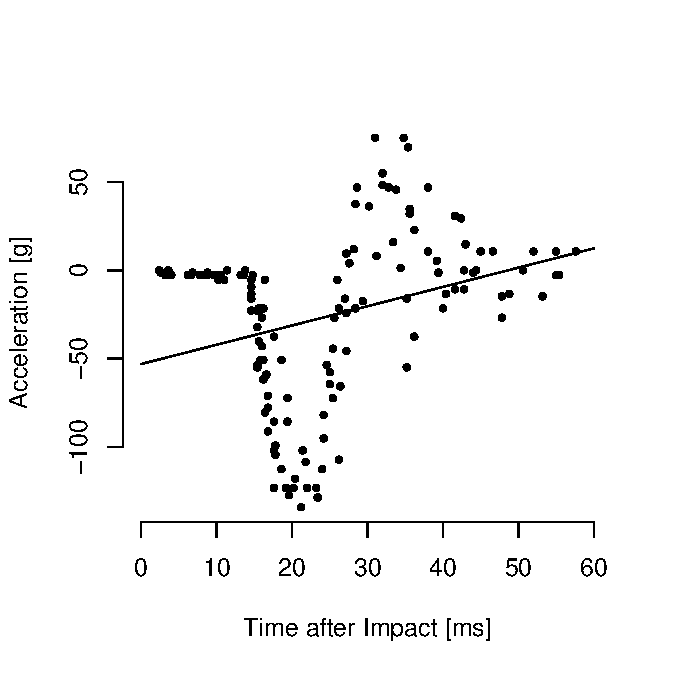
\includegraphics[width=\textwidth]{\FIGDIR/mcycle_p1}
    \caption{Linear regression}
  \end{subfigure}
	\hfill
	\begin{subfigure}[b]{0.45\textwidth}
    \centering
		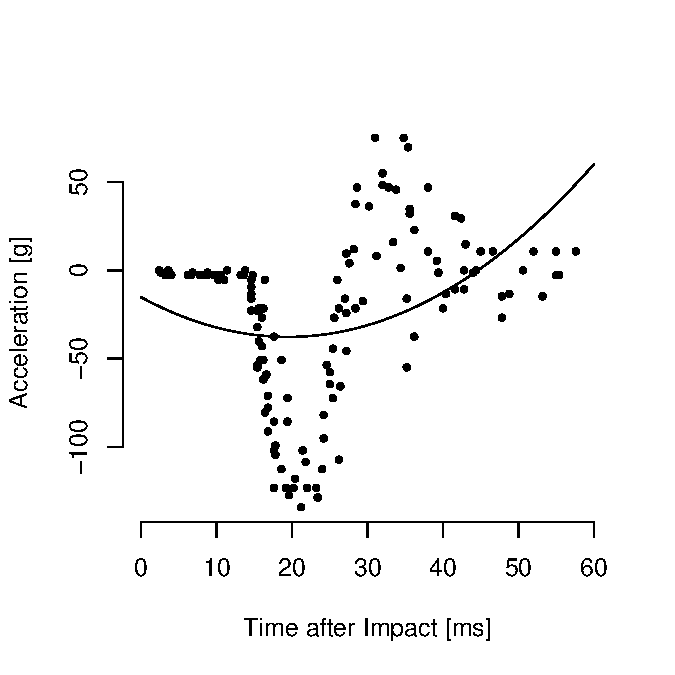
\includegraphics[width=\textwidth]{\FIGDIR/mcycle_p2}
    \caption{Quadratic regression}
  \end{subfigure}

	\begin{subfigure}[b]{0.45\textwidth}
    \centering
		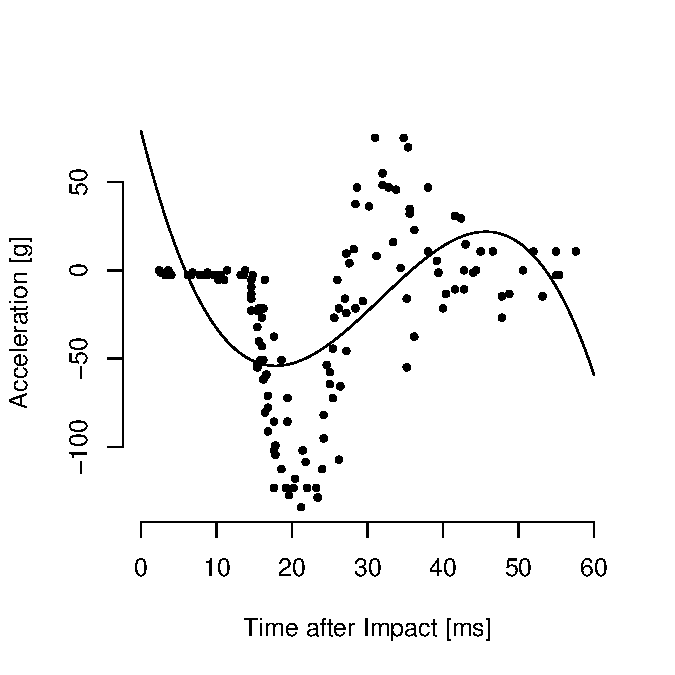
\includegraphics[width=\textwidth]{\FIGDIR/mcycle_p3}
    \caption{Kubic regression}
  \end{subfigure}
	\hfill
	\begin{subfigure}[b]{0.45\textwidth}
    \centering
		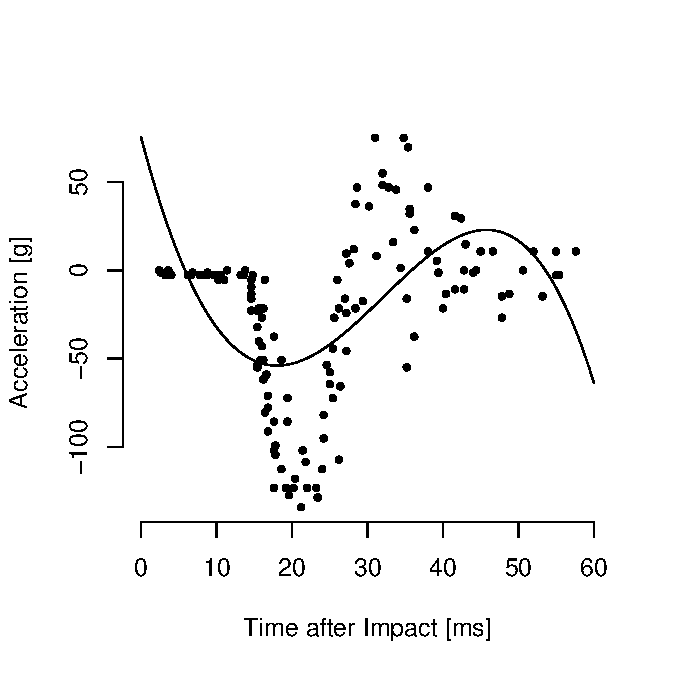
\includegraphics[width=\textwidth]{\FIGDIR/mcycle_p4}
    \caption{Quartic regression}
  \end{subfigure}

	\caption{Polynomial fits to the motorcycle data. The bias of estimates is large even in case of high-order polynomials. The plots are adapted from~\cite{Fan03}.}
	\label{fig:mcycle}
\end{figure}

Another solution is to estimate the objective function locally for each value $\x \in \mathcal{X}$. For that, we assign weights to individual observations based on their distance from $\x$. The further the point is, the lower the weight is. Also, it is possible to assign zero weights to observations from certain distance and exclude these points from estimation. Let us assign the weights to individual observations with a kernel function.

\begin{definition}
	Let $K: \R \to \R$ be a real function satisfying
	\[
		\int_{\R} K(x) dx = 1, \qquad
		\int_{\R} x K(x) dx = 0, \qquad
		0 < \int_{\R} x^2 K(x) dx < \infty
	\]
	Then we call $K$ a \emph{kernel function}.
\end{definition}

\cite{Cleveland79} proposed also other properties that a weight function should have. These are non-negativity, symmetry around zero, monotonicity for all non-negative values, and zero values outside the unit circle. The first three properties are fulfilled for the majority of common kernel functions. The fourth property is reasonable especially for computational purposes, but there are several kernel functions that violate this property. Later, we will see that symmetry of kernel function is unnecessary for our purpose.

Clearly, any density function of a non-degenerate random variable with zero mean and finite variance is a kernel function. Three common examples are the Gaussian kernel
\[
	K(x) = \frac{1}{\sqrt{2 \pi}} \exp \left( - \frac{x^2}{2} \right),
\]
the Epanechnikov kernel
\[
	K(x) = \begin{cases}
		\frac{3}{4} (1-x^2) \qquad & \text{if } \vert x \vert \leq 1 \\
		0 \qquad & \text{else,}
	\end{cases}
\]
and the Tricube kernel
\[
	K(x) = \begin{cases}
		\frac{70}{81} (1 - \left| x \right|^3)^3 \qquad & \text{if } \vert x \vert \leq 1 \\
		0 \qquad & \text{else.}
	\end{cases}
\]
The Tricube kernel was originally proposed by \cite{Cleveland79} and is implemented in R software, package stats, function loess.

Assume that the estimated function is $\mu (\x) = \E [ Y \vert \X = \x ]$. Then the \emph{local polynomial estimator} is in form of
\begin{equation}
	\label{eq:locReg}
	\begin{aligned}
		\widehat{\mu} (\x) = & \widehat{\varphi}_{\x} (\0) \\
		\widehat{\varphi}_{\x} = & \underset{\varphi}{\argmin} & & \sum_{i=1}^n K \left( \frac{ \left\| \X_i - \x \right\| }{h_{\alpha}(\x)} \right) (Y_i - \varphi (\X_i-\x))^2 \\
		& \st & & \varphi \text{ is a polynomial of degree } p.
	\end{aligned}
\end{equation}
Function $\left\| \cdot \right\|$ is the Euclidean norm of a vector. Function $h_{\alpha} (\x)$ is distance between $\x$ and $r$-th closest variable within $\X_1, ..., \X_n$, where $r = \left\lceil \alpha n \right\rceil$. By selecting the kernel function $K$ we control the weights of individual simulations. The span $\alpha$ and the degree $p$ of polynomial $\varphi$ are also of our choice.

We can use the estimated polynomial $\widehat{\varphi}_{\x}$ to estimate also derivatives of mean function by setting
\begin{align*}
	\widehat{\nabla_{\mu}} (\x) &= \nabla_{\widehat{\varphi}_{\x}} (\0), \\
	\widehat{\nabla_{\mu}^2} (\x) &= \nabla_{\widehat{\varphi}_{\x}}^2 (\0).
\end{align*}
For the gradient descent method, we need the local polynomial at least linear ($p \geq 1$). For the Newton's method, we need at least quadratic polynomials ($p \geq 2$).

Let us introduce a method that combines the gradient descent method and the Newton's method. We estimate the second-order derivative of the objective function only as a diagonal matrix. There are two main reasons for not estimating whole Hessian. First, the number of parameters that needs to be estimated is too high and the method is computationally demanding for high-dimensional problems. Second, the Newton's method needs the Hessian (or estimated Hessian) to be invertible. If the matrix is diagonal with non-zero diagonal elements, the inverse always exists. We can define the iterative method as
\begin{equation}
	\label{eq:hybridMethod}
	x^{(k+1)}_i =
		\begin{cases}
			x^{(k)}_i - \displaystyle{\frac {\widehat{\nabla}_{g,i} (\x^{(k)}_i)} {\widehat{\nabla}^2_{g,i,i} (\x^{(k)}_i)}},  & \widehat{\nabla}^2_{g,i,i} (\x^{(k)}_i) < -\frac{1}{\alpha_k} \\
			x^{(k)}_i + \alpha_k \widehat{\nabla}_{g,i} (\x^{(k)}_i), & \text{else,}
		\end{cases}
\end{equation}
where $\widehat{\nabla}_{g,i}$ and $\widehat{\nabla}^2_{g,i,i}$ denote the estimated derivatives of the objective function with respect to $x_i$. The condition on the first line of the definition of the next iteration has two reasons. First, we want to use the second derivatives only if the function is locally estimated as concave down. Second, we want to keep the algorithm stable even around estimated inflexion points where the estimated second derivative is close to zero.

\begin{algorithm}[Response Surface]\
	\label{algo:stochApprox}
	\begin{enumerate}
		\item Set initial value $\x^{(0)}$ and put $k := 0$.
		\item Generate data (multiple independent observations) from distribution $(\X, Y)$, where the predictors $\X$ have the distribution centered at $\x^k$. Join the data with previously generated data (if any).
		\item Fit the local polynomial regression at point $\x^{(k)}$. If the estimated first-order derivatives of $\mu$ are sufficiently close to zero then continue with step 5.
		\item Update $\x^{(k+1)}$ by~(\ref{eq:hybridMethod}) based on estimated derivatives, increase $k := k+1$ and repeat steps 2--4.
		\item Return value $\x^{(k)}$.
	\end{enumerate}
\end{algorithm}

Note that the algorithm does not return the estimated optimum of given problem. The reason for that is that local polynomial regression provides, in general, biased estimate of the estimated function. One can generate multiple observations from distribution $Y \vert \X = \widehat{\x}^{*}$.

Let us illustrate the method on simple example of finding an optimum of exponential of an paraboloid.

\begin{example}
	\label{ex:paraboloidSurface}
	Let $Y = \e^{- \left\| \x \right\|^2} + \varepsilon$, where $\x \in \R^2$ and $\varepsilon \sim N(0,1)$. Suppose that the optimization problem is
	\begin{equation*}
		\begin{aligned}
			& \underset{\x}{\max} & & \mu (\x) \\
			& \st & & \x \in \R^2.
		\end{aligned}
	\end{equation*}
	Clearly, the optimum is $\mu^{*} = 1$ at point $\x = (0,0)^{\top}$. However, we want to estimate the optimum using the Algorithm~\ref{algo:stochApprox}.
	
	We set the initial guess $\x^{(0)} = (1,1)^{\top}$ and at $k$-th iteration we generate 10~000 simulations with distribution of predictors as $\X \sim N_2 (\x^{(k)}, 0.01 \times \mathbb{I}_2)$, where $\mathbb{I}_2$ is $2 \times 2$ unit matrix. The sequence of steps lengths was defined as $\alpha_k = \frac{0.6}{\sqrt[3]{k+1}}$. At $k$-th iteration we used $\frac{0.75}{\sqrt{k+1}} \times 100\%$ nearest observations to fit the polynomial regression with Epanechnikov kernel as weights.
	
	The average distance of the estimated optimum from the actual optimum was 0.074 (confidence interval: 0.046--0.101). The mean number of iterations was 23.3. Some paths of the algorithm and all the estimated optimums are visualized in Figure~\ref{fig:paraboloidSurface}.
	
	\begin{figure}[t]
		\centering
		
			\begin{subfigure}[b]{0.45\textwidth}
				\centering
				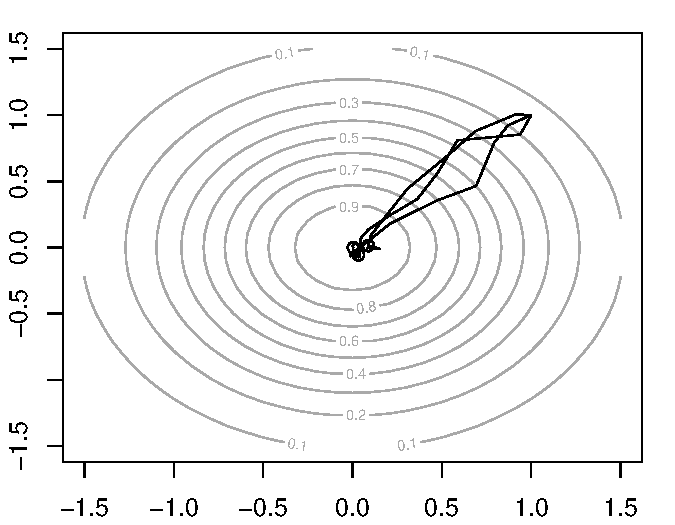
\includegraphics[width=\textwidth]{\FIGDIR/paraboloid_surface_path}
				\caption{Paths of three runs.}
			\end{subfigure}
			\hfill
			\begin{subfigure}[b]{0.45\textwidth}
				\centering
				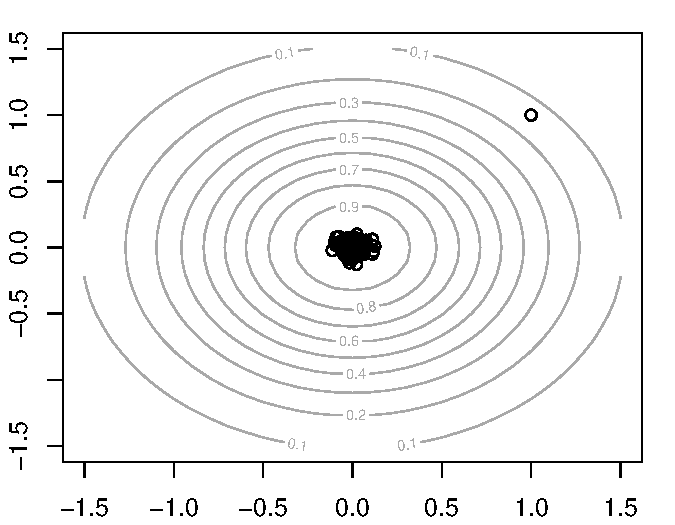
\includegraphics[width=\textwidth]{\FIGDIR/paraboloid_surface_endpoint}
				\caption{End points of 100 runs.}
			\end{subfigure}

		\caption{Visualized results of response surface method from Example~\ref{ex:paraboloidSurface}.}
		\label{fig:paraboloidSurface}
	\end{figure}

	\demo
\end{example}

Until now, we supposed only mean function as the objective function. The method can be generalized for various other functions. One can easily replace the local polynomial regression with any other local model. For example, by using the local quantile regression we can maximize the Value at Risk of random variable $Y \vert \X = \x$. For more local models that could be applied in the response surface method see~\cite{Fan03}.



%%%%%%%%%%%%%%%%%%%%%%%%%%%%%%%%%%%%%%%%%%%%%%%%%%%%%%%%%%%%%%%%%%%%%%%%%%%%%%%%%%%%%%%
%%%%%%%%%%%%%%%%%%%%%%%%%%%%%%%%%%%%%%%%%%%%%%%%%%%%%%%%%%%%%%%%%%%%%%%%%%%%%%%%%%%%%%%
\section{Cross Entropy Method}
	\label{chap:crossEntropy}
	
	Another way to find the optimum of given function with a noise is to use the cross entropy method. This method searches for the optimum by narrowing the set over which the objective function is optimized. In general, this method does not estimate the maximum of the conditional mean as the response surface method does. Also, only a little is known about the convergence of the algorithm.
	
	The algorithm has two main steps. In the first step, the independent values are generated from some distribution and the values that performs the best are selected for the second step. In the second step, the sampling distribution is updated based on the best performances from the first step. It is suitable to use the sampling distributions fixed up to the choice of the distribution parameter and update only the parameter.
	
	Following algorithm is adapted from \cite{Kroese11}.

\begin{algorithm}[Cross Entropy for Noisy Optimization]\
	\label{algo:crossEntropy}
	\begin{enumerate}
		\item Set initial parameter $\bm{\psi}^{(0)}$ and counter $k := 1$.
		\item Generate data (multiple independent observations) of size $n$ from distribution $(\X, Y)$, where the predictors have the distribution $\X \sim f( \;\cdot\; ; \bm{\psi}^{(k-1)})$. Let $\gamma_k$ be the $(1-\varrho)$-quantile of $Y_1, ..., Y_n$.
		\item Estimate the parameter $\bm{\psi}^{(k)}$ from the best performing observations using maximum likelihood
		\[
			\bm{\psi}^{(k)} = \underset{\psi}{\max} \sum_{\X_i \geq \gamma_k} \log ( f ( \X_i; \bm{\psi} ) ).
		\]
		\item If the distribution $f( \;\cdot\; ; \bm{\psi}^{(k)})$ is almost degenerated then continue with step 6, otherwise increase $k := k+1$ and repeat steps 2--4.
		\item Return value $\x$ such that the distribution $f( \;\cdot\; ; \bm{\psi}^{(k)})$ is almost degenerated at point $\x$.
	\end{enumerate}
\end{algorithm}

In the previous algorithm, the stopping criterion is vaguely described as \emph{almost degenerated distribution} $f( \;\cdot\; ; \bm{\psi})$. We use the 1-norm of the variance matrix of the distribution. If the norm is sufficiently close to zero we say that the distribution is almost degenerated.

To compare the algorithm with the response surface method, we use the cross entropy to solve the same problem as we did in previous chapter.

\begin{example}[Continuation of Example~\ref{ex:paraboloidSurface}]
	\label{ex:paraboloidCrossEntropy} 
	We choose to use bivariate normal distribution as the sampling distribution. We set the initial parameters for the distribution as $\mu = (1,1)^{\top}$ and $\sigma^2 = 5 \times \mathbb{I}_2$, where $\mathbb{I}_2$ is $2 \times 2$ unit matrix. The best performances in each iteration are selected using median, i.e. $\varrho = 0.5$.
	
	The average distance of the estimated optimum from the actual optimum was 0.036 (confidence interval: 0.033--0.038). The mean number of iterations was 28.2. Some paths of the algorithm and all the estimated optima are visualized in Figure~\ref{fig:paraboloidCE}.
	
	\begin{figure}[t]
		\centering
		
			\begin{subfigure}[b]{0.45\textwidth}
				\centering
				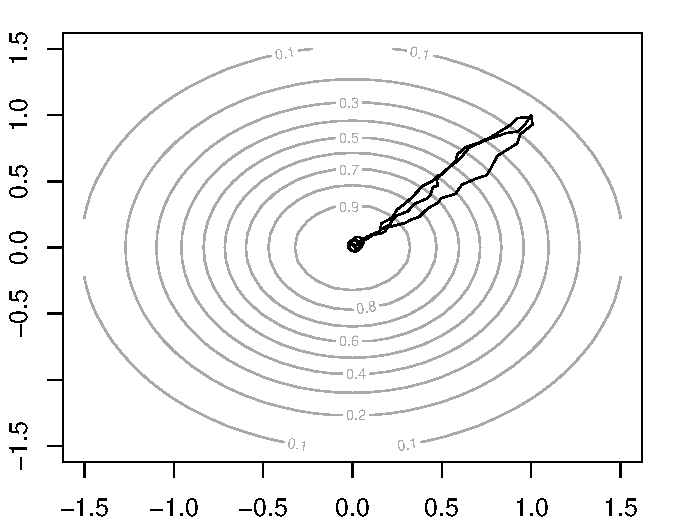
\includegraphics[width=\textwidth]{\FIGDIR/paraboloid_CE_path}
				\caption{Paths of three runs.}
			\end{subfigure}
			\hfill
			\begin{subfigure}[b]{0.45\textwidth}
				\centering
				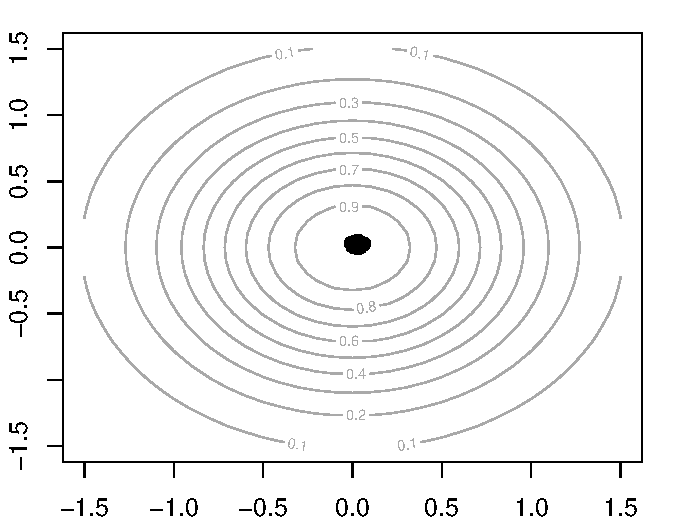
\includegraphics[width=\textwidth]{\FIGDIR/paraboloid_CE_endpoint}
				\caption{End points of 100 runs.}
			\end{subfigure}

		\caption{Visualized results of cross entropy method from Example~\ref{ex:paraboloidCrossEntropy}.}
		\label{fig:paraboloidCE}
	\end{figure}
		
	The cross entropy algorithm provided better results in only a few more iterations. Additionally, this method is computationally less demanding, because we do not need to estimate regression model at each iteration and we do not need to keep all the generated data.

	\demo
\end{example}

Another possibility is to combine both described methods. One could use the cross entropy method to find a solution that will be used as the initial point for the response surface method. By doing this, there are already generated data before the first iteration of the response surface algorithm. Also, the initial point might be closer to the actual solution than the initial guess would be.



%%%%%%%%%%%%%%%%%%%%%%%%%%%%%%%%%%%%%%%%%%%%%%%%%%%%%%%%%%%%%%%%%%%%%%%%%%%%%%%%%%%%%%%
%%%%%%%%%%%%%%%%%%%%%%%%%%%%%%%%%%%%%%%%%%%%%%%%%%%%%%%%%%%%%%%%%%%%%%%%%%%%%%%%%%%%%%%
\section{Multistage Optimization}
	\label{chap:multistage}

Until now, we considered only single-stage problems with one ($d$-dimensional) decision variable. In this chapter, we introduce a method for solving problems with several points in time when the decision has to be done. However, we still consider problems that need to be solved using one of the simulation method. We also need to add one variable to the model to track the history of the realized uncertainty. We considered general objective function $g$ for the simple problems. For the multistage problems we consider only mean function $g = \mu$ for the objective function.

For the $M$-stage stochastic problem we consider following assumptions. Let $\x_1, ..., \x_{M} \in \mathcal{X} \subset \R^d$ be the decision variables. Suppose that the constraints for the decision variable $\x_m$ depends on the very previous decision $\x_{m-1}$ for $m = 2, ..., M$. Denote the largest set that fulfills such constraints by $\mathcal{X} (\x_{m-1})$. Let $\varepsilon_1, ... \varepsilon_M$ be the sequence of random variables that we call the uncertainty of the problem. Suppose the uncertainty depends on the last decision. Then we talk about the \emph{endogenous uncertainty}. Let $\z_0, ..., \z_M \in \S$ be the random variables identifying the state of the decision model. Suppose the number of states is at most countable. The states depend on the very previous state, the last decision and the realization of the uncertainty. One can write $\z_m = \z_m (\z_{m-1}, \x_{m}, \varepsilon_m)$ for $m = 1, ..., M$. Since the state has a random variable as an argument it is random itself as well and it is natural to talk about its distribution. The state $\z_0$ is known (deterministic) prior to the first decision. The dynamics of the model is illustrated in Figure~\ref{fig:dynamics}~(a).

\begin{figure}[t]
	\centering
	
		\begin{subfigure}[b]{\textwidth}
			\centering
			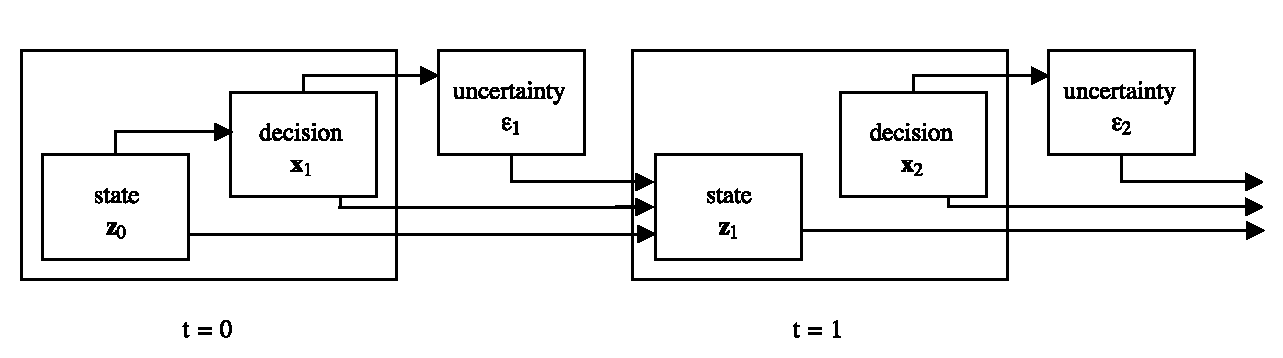
\includegraphics[width=\textwidth]{\FIGDIR/diagramEndogenous}
			\caption{Endogenous uncertainty.}
		\end{subfigure}
		%\vspace*{150px}
		\begin{subfigure}[b]{\textwidth}
			\centering
			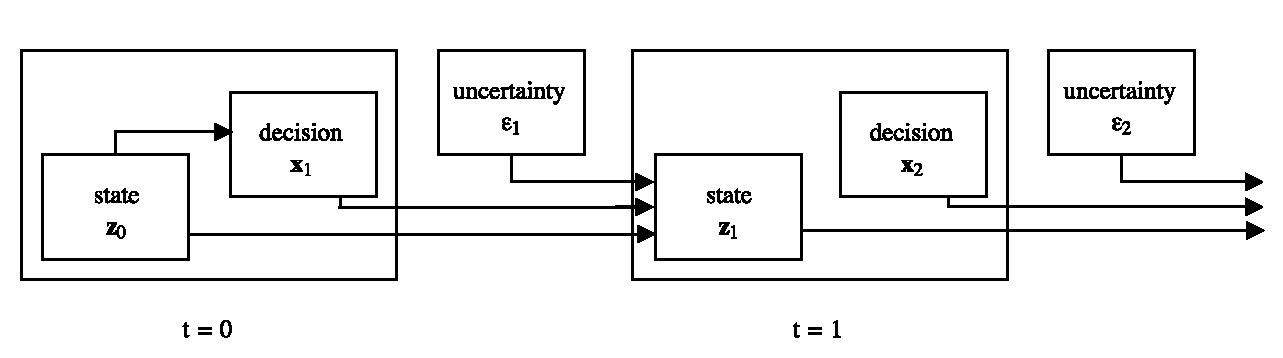
\includegraphics[width=\textwidth]{\FIGDIR/diagramExogenous}
			\caption{Exogenous uncertainty.}
		\end{subfigure}

	\caption{Comparison between the dynamics of the state-space decision model with endogenous and exogenous uncertainty. Adapted from \cite{Pflug14}.}
	\label{fig:dynamics}
\end{figure}

Let the objective random variables be denoted by $Y_m = h (\z_m, \z_{m-1}, \x_{m})$ for $m=1, ..., M$, where $h: \R^{2c+d} \to \R$ is a measurable function. The variable $Y_m$ is usually called a \emph{transition reward}. Denote the expected reward in the $m$-th time interval by $g_{m} (\x_{m}, \z_{m-1}) = \E [Y_m \vert \x_{m}, \z_{m-1}]$. Let the multistage problem be
\begin{equation}
	\label{eq:multistageMax}
	\begin{aligned}
		G_0 = & \underset{\x_1, ..., \x_{M}}{\max} & & \sum_{m=1}^M  g_m (\x_{m}, \z_{m-1})\\
		& \st & & \x_1 \in \mathcal{X}, \\
		&  		& & \x_m \in \mathcal{X} (\x_{m-1}), \qquad m = 2, ..., M.
	\end{aligned}
\end{equation}
Similarly, we can write recursive problems for $m = 1, ..., M-1$
\begin{equation}
	\label{eq:recursiveMax}
	\begin{aligned}
		G_m (\x_{m}, \z_{m}) = & \underset{\x_{m+1}, ..., \x_{M}}{\max} & & \sum_{k=m+1}^M  g_k (\x_{k}, \z_{k-1})\\
		& \st & & \x_k \in \mathcal{X} (\x_{k-1}), \qquad k = m, ..., M.
	\end{aligned}
\end{equation}
Note the state $\z_{m}$ is unknown (depends on unobserved the uncertainty $\varepsilon_{m}$) at time $m$ and, therefore, is random. Since the problem~(\ref{eq:recursiveMax}) depends on $\z_{m}$ it is random as well. \cite{Pflug14} showed that the problem~(\ref{eq:multistageMax}) is equivalent to
\begin{equation}
	\label{eq:reformMax}
	\begin{aligned}
		& \underset{\x_1, ..., \x_{M}}{\max} & & g_1 (\x_{1}, \z_{0}) + \E [G_1 (\x_{1}, \z_{1})] \\
		& \st & & \x_0 \in \mathcal{X}.
	\end{aligned}
\end{equation}

Suppose that we are able to evaluate (generate random variable from such distribution) the function $G_1 (\x_{1}, \z_{1})$. Then we can use some of the method described in Chapters~\ref{chap:responseSurface} and~\ref{chap:crossEntropy} to find the optimum of~(\ref{eq:reformMax}).

Evaluation of $Q_1 (\x_{0}, \z_{1})$ consists of two parts: generating the uncertainty $\varepsilon_1$ and solving the stochastic problem with $M-1$ stages and known initial state $\z_1 (\varepsilon_1)$. If $M=2$ then the problem is easy to solve. For larger problems we need to iterate through the procedure until the problem at the end is single-stage.




\part{Practical Applications}
	\chapter{Stochastic Demand}
	\label{chap:Demand}

In this chapter, we introduce a model for stochastic demand for a service with limited inventory and clearly bounded time when the service may be sold. We also propose a method for estimating the parameters of the demand. The model is illustrated on example of train tickets.

Suppose that the demand follows Poisson distribution with intensity $\Lambda (p)$, where $p$ is the price. Denote the period when the service is being sold by $[0, T]$. Assume there exists positive intensity function $\lambda (p,t)$ that identifies the change of the demand during time. It has to hold that $\Lambda (p) = \int_0^T \lambda (p,t) dt$. In this example we suppose the demand intensity has the elasticity constant in price and linear in time. Constant elasticity functions are widely used in microeconomics. \cite{Williams13} investigated the data from airline ticket prices and concluded that passengers are more likely to accept high prices as the departure time encloses. Function with mentioned attributes may be
\begin{equation}
	\label{eq:demandModel}
	\lambda (p, t; \m{\beta}) = \exp (\beta_1 + \beta_2 \log (p) + \beta_3 t + \beta_4 t \log (p)),
\end{equation}
for which the price elasticity is
\[
	\frac{\partial \lambda (p,t; \m{\beta})}{\partial p} \frac{p}{\lambda (p,t)} = \beta_2 + \beta_4 t.
\]
Note that the intensity lacks any periodicity (daily, weekly, etc.). This model is, however, able to capture the trend in demand intensity which is the most important part. The imperfection of the model is balanced by computational speed. This will become more clear in Chapter~\ref{chap:optimalPrice} where we need the inverse function of the cumulative intensity to simulate the demand.

This model for demand may be used for the tickets for each route (the pair of boarding and exiting stations). It is possible to assume that some of the parameters may be the same for each route or some group of routes, e.g. one can assume that the elasticity is the same for routes with similar route length. We do not make any assumptions about the relations between parameters of individual routes. Further, we assume that the demands for individual routes are mutually independent.

This market for train tickets is specific in following ways:
\begin{enumerate}[\itshape i)]
	\item The tickets can be sold only up to given time (departure of the train). This time is different for each boarding station.
	\item The inventory level (number of seats available) is set before the tickets are purchased and cannot be changed dynamically.
	\item There exists a rivalry between customers even if they are purchasing different service. Such case may happen when two passengers have no station (nor boarding or exiting) in common, but their journeys have an intersection. These passengers cannot buy the ticket for the same seat in the train. This implies that the number of seats available is random for each par of boarding and exiting station. The reservation system may be managed in one of the following ways.
	\begin{enumerate}[a)]
		\item The passenger may choose any of the seats that is available for whole his route. If there is no such seat, the ticket is unavailable for the route.
		\item The system selects the seat that would provide the best seating availability for upcoming passengers and sends the seat number to the passenger at the time of the purchase.
		\item The system sends the seat number to the passenger right before the train departures (e.g. at the time the purchasing period is over).
	\end{enumerate}
	The model we introduce in this thesis is applicable to system~c). System~b) requires additional combinatorial optimization for seat selection. System~a) may result in significant revenue losses due to ineffectiveness in allocation of seats to passengers.
	\item The tickets may be in some cases returned to the seller (depends on the conditions of individual carrier). The customer has to pay a ratio of original price as a cancellation fee, say $r \in [0,1]$. In our example, the ticket cannot be returned, i.e. $r = 1$.
	\item The service is provided in classes that differ in price and number of supplementary services. The demand for each class should be modeled individually. The price elasticity is usually lower (higher in absolute value) for higher classes. We suppose only one class in the train.
	\item There are several passenger types with different demands. In some countries, the carrier is obliged\footnote{For example based on Assessment Notice 01/2016 of Ministry of Finance of the Czech Republic.} to make a discount for some of the passenger types (e.g. students, seniors, handicapped person, etc.). We suppose only one passenger type.
\end{enumerate}

Suppose the train goes through $K$ stations (including the first and the last one) and $M$ seats. Denote these stations by $\{1, ..., K\}$. Since the arrivals of passengers for each route follow inhomogeneous Poisson process and the upper bound for the number of passengers depends on the demand for tickets for different routes it is suitable to model number of passengers for all routes with an inhomogeneous Markov process. The states identify number of tickets sold for each route, i.e. the state space $\S$ is $\binom{K}{2}$-dimensional with values in $\N_0$. Even though it is possible to index the dimensions of the states with only one number (e.g. $s_i$ would be the number of passengers for $i$-th route for state $\m{s} \in \S$, where $i \in \{1, ..., \binom{K}{2} \}$) we index the dimensions with two numbers denoting the boarding and exiting station (e.g. $s_{k,l}$ is the number of passengers traveling on the route $(k,l)$ from station $k$ to station $l$, where $k,l \in \{1, ..., K\}$ and $l > k$). The initial state denoting empty train is $\m{0} = (0, ..., 0)$. Similarly, we denote the prices as a $\binom{K}{2}$-dimensional vector $\m{p}$ with indexes $\{ (k,l): 1 \leq k < l \leq K \}$.

There is a capacity condition that every state of the state space must fulfill, i.e.
\[
	\S = \left\{ \s \in \N_0^{\binom{K}{2}}: \sum_{k=1}^h \sum_{l=h+1}^K s_{k,l} \leq M, \forall h = 1, ..., K-1 \right\}
\]
Denote by $\omega (\s, k, l)$ the state which the system transitions into after arrival of a passenger for route $(k,l)$ when the system was in state $\s \in \S$. It is clear that
\[
	\omega (\s, k, l) = \s + \omega (\0, k, l).
\]
The state $\omega (\s, k, l)$ is an element of state space $\S$ if and only if there is an empty seat for route $(k,l)$ is state $\s \in \S$. The transition intensity from state $\s \in \S$ to state $\omega (\s, k, l) \in \S$ is equal to $\lambda_{k,l}$, i.e. the demand intensity for route $(k,l)$. The total transition intensity from state $\s \in \S$ at time $t \in [0,T]$ with prices $\m{p}$ is given by
\[
	q_{\s} (\m{p}, t; \m{\beta}) = \sum_{k=1}^{K-1} \sum_{l=k+1}^K \lambda_{k,l} (p_{k,l}, t, ; \m{\beta}_{k,l}) \times \mathbb{I} [ \omega (\s, k, l) \in \S ],
\]
where $\m{\beta}_{k,l} = (\beta_{1,k,l}, ..., \beta_{4,k,l})^{\top}$ denotes the parameters that matter for route $(k,l)$ and
\[
	\bm{\beta} = \{ \beta_{h,k,l}: 1 \leq h \leq 4, 1 \leq k < l \leq K \}
\]
denotes the aggregated parameter of the demand.

Suppose we have the data from selling system from $n$ trains with equal demands (e.g. trains at the same time and day in week in multiple consequence weeks). Denote by $N^{\nu}$ the number of passengers in $\nu$-th train. Use following notation for the observed data about $i$-th passenger in $\nu$-th train:
\begin{center}
	\begin{tabular}{ll}
		T_i^\nu & purchase time, \\
		p_i^\nu & price of the ticket, \\
		(k_i^\nu, l_i^\nu) & route (boarding station, exiting station).
	\end{tabular}
\end{center}

Suppose that the price was constant over $J$ time intervals that were the same for each train. Denote by $[ \tau_{j-1}, \tau_j ]$ the interval over which the price $\m{p}^{(j)}$ was effective for $j = 1, ..., J$. Denote by $\hat{\tau}_{k,l}^{\nu}$ the time the tickets for route $(k,l)$ on train $\nu$ became unavailable due to the capacity limitations or due to the departure of the train.

Let us denote a set of passengers that travel route $(k,l)$ for each train by
\[
	\mathcal{I}_{k,l}^{\nu} = \left\{ i \in \{ 1, ..., N^{\nu} \} : k_i^\nu = k, l_i^\nu = l \right\}.
\]
The elements of the score function~(\ref{eq:finalU}) that matter for route $(k,l)$ can be written as
\begin{multline*}
	\m{U}_{n,k,l} (\m{\beta})
	= \sum_{\nu=1}^{n} \\
	\left[ \sum_{i \in \mathcal{I}_{k,l}^{\nu}} \left(
		\begin{array}{c}
			1 \\ \log(p_i^\nu) \\ T_i^\nu \\ T_i^\nu \log(p_i^\nu)
		\end{array}
	\right) - 
	\sum_{j=1}^J \int_{\tau_{j-1}}^{\tau_j} \m{V}_{k,l}^{(j)} (t) \; \lambda_{k,l} (p_{k,l}^{(j)}, t; \m{\beta}_{k,l}) \; \mathbb{I} [t < \hat{\tau}_{k,l}^{\nu}] dt \right],
\end{multline*}
where
\[
	\m{V}_{k,l}^{(j)} (t) = \left(
		\begin{array}{c}
			1 \\ \log(p_{k,l}^{(j)}) \\ t \\ t \log(p_{k,l}^{(j)})
		\end{array}
	\right).
\]
The observed information matrix~(\ref{eq:finalI}) is block diagonal. The block that matters for route $(k,l)$ is
\[
	\m{I}_{n,k,l} (\m{\beta}) = \frac{1}{n} \sum_{\nu=1}^{n} \left[
	\sum_{j=1}^J \int_{\tau_{j-1}}^{\tau_j}
	\left(\m{V}_{k,l}^{(j)} (t)  \right)
	\left(\m{V}_{k,l}^{(j)} (t)  \right)^{\top}
	\lambda_{k,l} (p_{k,l}^{(j)}, t; \m{\beta}_{k,l})
	\; \mathbb{I} [t < \hat{\tau}_{k,l}^{\nu}] dt \right].
\]
The estimate $\hat{\m{\beta}}_n$ needs to be found using Newton-Raphson method described in Chapter~\ref{chap:statistics}.

Note that even though the variance matrix of the estimate $\hat{\m{\beta}}_n$ is block diagonal the elements of the estimate that matter for different routes are still dependent. The seat availability determined by passengers on all routes influences the variance of the estimate.

The method was used for an analysis of simulated data of processes of selling the tickets for 500 trains. The demand was both simulated and estimated using model~(\ref{eq:demandModel}). The parameters for demand intensity for each route individually are in Table~\ref{tab:estimatedBeta}. The tickets began to sell 60 days before the departure, say at time $0$. For computational purposes we assume the time period of 60 days as $[0,1]$. The train departed (and the tickets ended sells) from stations $1, ..., 5$ at times $\frac{59.4}{60}$, $\frac{59.44}{60}$, $\frac{59.48}{60}$, $\frac{59.52}{60}$, $\frac{59.56}{60}$, and $\frac{59.6}{60}$. Prices that we used for the simulations are in Table~\ref{tab:ticketPrices}. The times of price changes were at the end of the 30th, 46th, 54th, and 58th day.

Distribution of times of purchases is showed in Figure~\ref{fig:histTimes}. There are significant drops in demand right after the price has increased. Also at the end of the selling period the number of tickets sold decreases because the train departed from its begging station and some of the tickets cannot be sold anymore.

\begin{table}[ht]
	\centering
	\begin{tabular}{llllll}
		\hline
		route & $\m{p}^{(1)}$ & $\m{p}^{(2)}$ & $\m{p}^{(3)}$ & $\m{p}^{(4)}$ & $\m{p}^{(5)}$ \\ 
		\hline
		(1,2) & 110 & 121 & 133 & 146 & 161 \\ 
		(1,3) & 205 & 226 & 248 & 273 & 301 \\ 
		(1,4) & 296 & 325 & 358 & 394 & 433 \\ 
		(1,5) & 383 & 421 & 463 & 510 & 561 \\ 
		(1,6) & 468 & 515 & 567 & 623 & 686 \\ 
		(2,3) & 110 & 121 & 133 & 146 & 161 \\ 
		(2,4) & 205 & 226 & 248 & 273 & 301 \\ 
		(2,5) & 296 & 325 & 358 & 394 & 433 \\ 
		(2,6) & 383 & 421 & 463 & 510 & 561 \\ 
		(3,4) & 110 & 121 & 133 & 146 & 161 \\ 
		(3,5) & 205 & 226 & 248 & 273 & 301 \\ 
		(3,6) & 296 & 325 & 358 & 394 & 433 \\ 
		(4,5) & 110 & 121 & 133 & 146 & 161 \\ 
		(4,6) & 205 & 226 & 248 & 273 & 301 \\ 
		(5,6) & 110 & 121 & 133 & 146 & 161 \\ 
		 \hline
	\end{tabular}
	\caption{Prices for individual time periods used in simulation of demand for train tickets.}
	\label{tab:ticketPrices}
\end{table}

\begin{figure}[t]
	\centering
	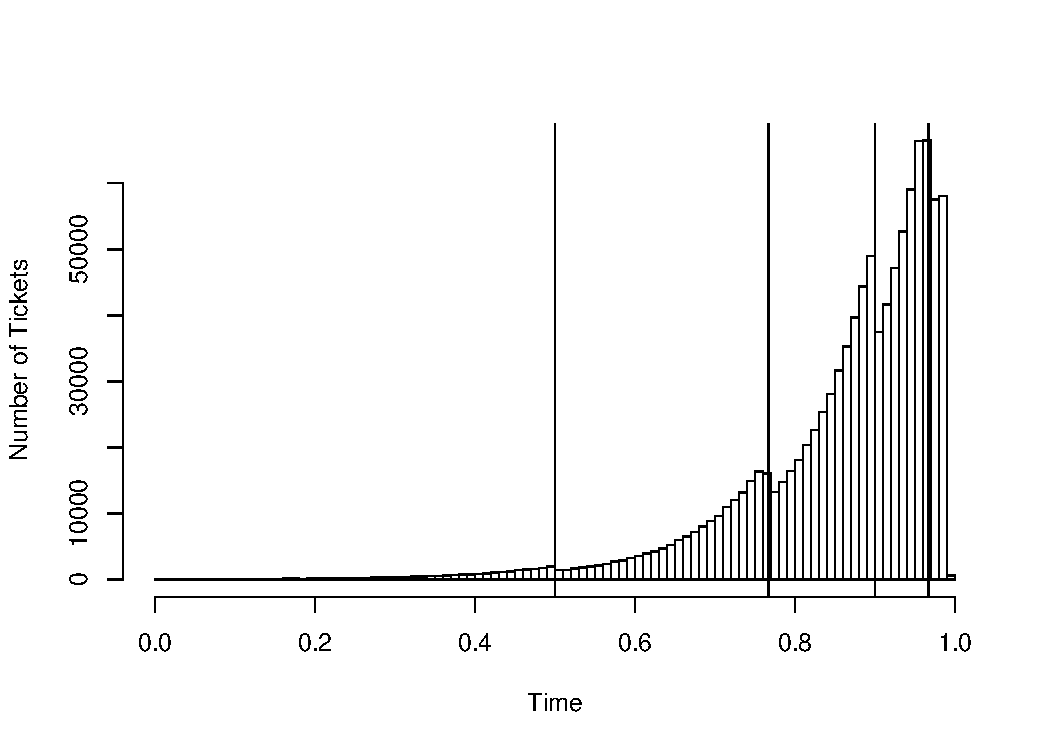
\includegraphics[width=0.85\textwidth]{figures/histTimes.pdf}
	\caption{Histogram of times of purchase over all simulated trains. Vertical lines indicate the times of price changes.}
	\label{fig:histTimes}
\end{figure}

% latex table generated in R 3.3.0 by xtable 1.8-2 package
% Fri Jul 22 14:17:54 2016
\begin{sidewaystable}[p]
\centering
\begin{tabular}{c|cccc|cccc|cccc|cccc}
  \toprule
				& \multicolumn{4}{c|}{Intercept} & \multicolumn{4}{c|}{\log(price)} & \multicolumn{4}{c|}{$time$} & \multicolumn{4}{c}{$time \times \log(price)$} \\
	route & act & est & 2.5\% & 97.5\% & act & est & 2.5\% & 97.5\% & act & est & 2.5\% & 97.5\% & act & est & 2.5\% & 97.5\% \\ 
  \midrule
	(1,2) & 18.37 & 18.385 & 17.523 & 19.247 & -4.19 & -4.207 & ~-8.456 & ~0.042 & 3.48 & 3.712 & ~2.965 & 4.459 & 1.14 & 1.109 & -2.589 & 4.808 \\ 
  (1,3) & 20.12 & 18.942 & 17.879 & 20.005 & -3.94 & -3.714 & ~-9.618 & ~2.190 & 3.49 & 4.478 & ~3.559 & 5.398 & 0.99 & 0.795 & -4.331 & 5.922 \\ 
  (1,4) & 23.00 & 25.247 & 23.872 & 26.622 & -4.25 & -4.641 & -12.792 & ~3.511 & 3.88 & 1.398 & ~0.192 & 2.603 & 1.04 & 1.472 & -5.703 & 8.647 \\ 
  (1,5) & 20.08 & 19.978 & 19.065 & 20.891 & -3.72 & -3.696 & ~-9.347 & ~1.955 & 3.83 & 3.487 & ~2.684 & 4.290 & 0.99 & 1.037 & -3.953 & 6.026 \\ 
  (1,6) & 22.67 & 21.758 & 20.816 & 22.699 & -3.90 & -3.764 & ~-9.774 & ~2.246 & 3.74 & 4.480 & ~3.662 & 5.299 & 0.86 & 0.752 & -4.491 & 5.995 \\ 
  (2,3) & 18.67 & 21.881 & 21.175 & 22.587 & -4.25 & -4.934 & ~-8.408 & -1.461 & 3.87 & 1.814 & ~1.210 & 2.417 & 0.96 & 1.419 & -1.567 & 4.404 \\ 
  (2,4) & 20.53 & 21.871 & 20.842 & 22.900 & -4.05 & -4.305 & -10.022 & ~1.412 & 3.81 & 2.815 & ~1.924 & 3.707 & 0.96 & 1.155 & -3.818 & 6.127 \\ 
  (2,5) & 20.80 & 20.658 & 19.893 & 21.424 & -3.98 & -3.971 & ~-8.506 & ~0.565 & 3.53 & 3.903 & ~3.236 & 4.570 & 0.99 & 0.942 & -3.025 & 4.910 \\ 
  (2,6) & 20.73 & 21.017 & 20.259 & 21.775 & -3.83 & -3.889 & ~-8.578 & ~0.800 & 2.70 & 3.551 & ~2.888 & 4.214 & 1.11 & 0.986 & -3.129 & 5.102 \\ 
  (3,4) & 17.97 & 16.491 & 15.595 & 17.387 & -4.09 & -3.775 & ~-8.191 & ~0.641 & 3.75 & 5.342 & ~4.567 & 6.117 & 1.08 & 0.742 & -3.097 & 4.582 \\ 
  (3,5) & 18.72 & 17.127 & 16.253 & 18.000 & -3.75 & -3.457 & ~-8.307 & ~1.393 & 3.48 & 5.417 & ~4.661 & 6.173 & 0.98 & 0.626 & -3.592 & 4.844 \\ 
  (3,6) & 21.20 & 24.279 & 23.126 & 25.433 & -3.88 & -4.415 & -11.245 & ~2.415 & 3.44 & 0.353 & -0.648 & 1.354 & 0.97 & 1.507 & -4.447 & 7.462 \\ 
  (4,5) & 18.54 & 13.776 & 13.139 & 14.412 & -4.19 & -3.163 & ~-6.292 & -0.034 & 2.91 & 6.586 & ~6.046 & 7.126 & 1.07 & 0.255 & -2.417 & 2.927 \\ 
  (4,6) & 23.62 & 19.962 & 19.048 & 20.875 & -4.66 & -3.963 & ~-9.035 & ~1.109 & 3.31 & 6.219 & ~5.432 & 7.005 & 1.06 & 0.495 & -3.889 & 4.880 \\ 
  (5,6) & 17.18 & 19.498 & 18.275 & 20.721 & -3.66 & -4.153 & -10.174 & ~1.868 & 3.67 & 1.525 & ~0.478 & 2.572 & 0.93 & 1.391 & -3.794 & 6.575 \\ 
   \bottomrule
\end{tabular}
\caption{Comparison of actual parameters of the demand intensity (act), their estimates (est), and boundaries of $95\%$ confidence interval ($2.5\%$, $97.5\%$) based on Wald test statistic.}
\label{tab:estimatedBeta}
\end{sidewaystable}


The number of simulated trains is clearly way higher that the railways company may be using for modeling the demand of single train. The assumption that the demand is the same for almost ten years is most certainly wrong. On the other hand, the demand for specific train might be similar to other trains departing in similar times or the same type of day in a week (workday or weekend) or the train in opposite direction. If the company dispatches for example 16 trains a day in each direction the total number of trains in a week is 224. That is why the number of simulated trains may be reasonable.

%Denote by $D_{s_0, s_1, t}$ the number of demanded tickets for the route from station $s_0$ to station $s_1$ up to time $t$. Under the assumptions it holds that $D_{s_0, s_1, t} \sim Poi (\Lambda(t))$, where $\Lambda(t)$ is unknown cumulative intensity. The processes $\m{D}_{s_0, s_1}$ are independent by assumption. The total number of sold tickets for individual routes cannot be modeled separately, because of the rivalry on the demand side.

%Denote by $\mathcal{A}$ the set of all stations for current train and by $\procX$ the multidimensional process containing the number of sold tickets for each pair of stations. Each dimension of the process indicates number of sold tickets for single pair of boarding and exiting station. Denote by $\lambda_{s_0, s_1}$ the intensity of process $\m{D}_{s_0, s_1}$. The transition intensities from state $i$ to state $j$ are given by $q_{ij} (t) = \lambda_{s_0, s_1}$ if the transition between such states is equivalent to arrival of one customer buying a ticket from station $s_0$ to station $s_1$. If all the seats are taken for such route, or the transition is not equivalent to any of such events, the transition intensity is zero. Denote by $\mathcal{A}_i^2 \subset \mathcal{A} \times \mathcal{A}$ all pairs of stations $(s_0, s_1)$ such that the ticket from $s_0$ to $s_1$ is available at state $i$. Denote by $\S_i \subset \S$ the set of all states directly accessible from state $i \in \S$ Denote by $r: \S \times \S \to \mathcal{A} \times \mathcal{A}$

	\chapter{Optimal Price of Fare}
	\label{chap:optimalPrice}
	
We use the demand intensity from previous chapter to find an optimal price of fare. First, we solve the single-stage problem to find the optimal price for each route that would apply for the whole selling period. Then we add the possibility to change the initial decision on the price during the selling period. The decision can be done only at certain moments, \emph{decision times}. The decision times are chosen before the selling period and cannot be change later.

The objective function to which the price is optimized is expected return, that is the sum of prices of all sold tickets. We use the same state space $\S$ as we did in Chapter~\ref{chap:Demand}. The objective variable for each stage of the multistage problem is
\[
	Y_m = h (\z_m, \z_{m-1}, \m{p}_{m}) = \m{p}_{m}^{\top} (\z_m - \z_{m-1}),
\]
where $\m{p}_m$ is the decision variable for $m$-th stage, i.e. the prices for all stations for $m$-th period. The randomness of $Y_m$ is caused via $\z_m$ (number of tickets sold at the end of $m$-th period) which depends on the uncertainty factor $\varepsilon_m$ (i.e. the randomness in demand).

The set of general feasible solutions $\mathcal{X}$ that must hold for prices between each decisions is given by following constraints:
\begin{enumerate}[\itshape i)]
	\item If one route is part of another route the longer route must not have cheaper tickets, i.e.
		\begin{equation}
			\label{eq:constr1}
			p_{k,l} \leq p_{k',l'}, \qquad k' \leq k < l \leq l'.
		\end{equation}
	
	\item A route must not have more expensive ticket than sum of ticket prices of routes that combine to the original route, i.e.
		\begin{equation}
			\label{eq:constr2}
			p_{k,l} \leq p_{k,h} + p_{h,l}, \qquad k < h < l.
		\end{equation}
	
	\item All tickets must have positive price. Due to condition \textit{i} it is sufficient to have only constraints on the routes between adjacent stations, i.e.
		\[
			p_{k,k+1} > 0, \qquad k = 1, ..., K-1.
		\]
		Since $\lambda (p, t; \m{\beta}) \to \infty$ as $p \to 0$ for reasonable values of $\m{\beta}$ ($\beta_2 + \beta_4 t < 0$) and the demand is simulated as Poisson process with such intensity, it is reasonable to forbid prices close to zero. Because of that we set constraints to
		\begin{equation}
			\label{eq:constr3}
			\m{p} \geq \m{p}_0,
		\end{equation}
		where $\m{p}_0 > 0$ is $\binom{K}{2}$-dimensional constant (in our case $\theta = (50, ..., 50)^\T$). 
\end{enumerate}
Constraints (\ref{eq:constr1}) and (\ref{eq:constr2}) are replaced by linear penalty function
\[
	\Phi_1 (\m{p}) =
		\displaystyle{\sum_{k' \leq k < l \leq l'}} [p_{k',l'} - p_{k,l}]_{_{+}} +
		\displaystyle{\sum_{k < h < l}} [p_{k,h} + p_{h,l} - p_{k,l}]_{_{+}}
\]
where $[\; \cdot \;]_{_{+}} = \max\{ \; \cdot \; , 0 \}$ denotes the positive part and $\bm{1}$ is vector of ones with respective length.
%The reason for the perfect penalty is that we are unable to simulate demand for negative or zero price and regardless the outcome of the $Y$ the objective function including the penalty function will be $-\infty$.

The specific conditions for $m$-th decision variables is given by
\begin{equation}
	\label{eq:constr4}
	\mathcal{X} (\m{p}_{m-1}) = \{ \m{p}_m \in \mathcal{X}: \m{p}_m \geq \m{p}_{m-1} \}, \qquad m = 2, ..., M
\end{equation}
so the tickets are at least that expensive as they were after previous decision. The penalty function for constraints (\ref{eq:constr3}) and (\ref{eq:constr4}) is
\[
	\Phi_2 (\m{p}_m) = \bm{1}^{\top} [\m{p}_{m-1} - \m{p}_m]_{_{+}}.
\]

We can write the maximization problem using penalty functions as
\begin{equation*}
	\begin{aligned}
		& \underset{\m{p}_1, ..., \m{p}_M}{\max} & & \E [\m{p}_{m}^{\top} (\z_m - \z_{m-1})] - \theta \left[ \sum_{m=1}^M \Phi_1 (\m{p}_m) + \sum_{m=2}^M \Phi_2 (\m{p}_m) \right] \\
		& \st & & \m{p}_m \in \R^{\binom{K}{2}}, \qquad m = 1, ..., M
	\end{aligned}
\end{equation*}
where $\theta > 0$ is a \emph{penalty coefficient}. In our case, we set $\theta = 1000$.




%%%%%%%%%%%%%%%%%%%%%%%%%%%%%%%%%%%%%%%%%%%%%%%%%%%%%%%%%%%%%%%%%%%%%%%%%%%%%%%%%%%%%%%
%%%%%%%%%%%%%%%%%%%%%%%%%%%%%%%%%%%%%%%%%%%%%%%%%%%%%%%%%%%%%%%%%%%%%%%%%%%%%%%%%%%%%%%
\section{Single-stage model}
	\label{chap:singleStageModel}

Let us begin with the single-stage problem, that is $M=1$ and the selected prices hold during whole selling period. The problem is solved in two phases. In the first phase, we use the cross entropy algorithm to find a solution that is close to the actual optimum. The algorithm is useful to begin with if we have no good guess where the solution is because it searches through the set of feasible solutions globally and narrows this set. On the other hand, it does not have to converge to the actual optimum. We used normal distribution as the sampling distribution. The initial mean is as in Table~\ref{tab:priceSolutions} (a) and the initial variance matrix is diagonal with diagonal elements $\sigma_{(k,l), (k,l)}^2 = 500$. The algorithm was iterated 20-times and during each iteration 2000 new data point were generated. New sampling distribution was estimated using $25\%$ best performing observations. The result of the algorithm is in Table~\ref{tab:priceSolutions} (b).

In the second phase, we used the response surface algorithm on the data generated in the first phase. In addition, we generated 500 new data during each iteration of the algorithm. The prices were generated from multivariate (mutually independent) normal distribution with mean equal to current approximation of the optimum price and standard deviation $10$. The derivative of the objective function was estimated locally using $30\%$ of the observations. The new approximation of the price were calculated by
\[
	\m{p}^{(r+1)} = \m{p}^{(r)} + \frac{\widehat{\nabla} (\m{p}^{(r)})}{20}.
\]
Results for this method are in Table~\ref{tab:priceSolutions} (c). Note that the solution does not fulfill the constraints~\eqref{eq:constr1}. This solution may be justified by projection into the set of feasible solutions.

\begin{table}[t]
	\centering
	
	\begin{subtable}[b]{0.49\textwidth}
    \centering
			\begin{tabular}{cccccc}
				\hline
					& 2 & 3 & 4 & 5 & 6 \\ 
				\hline
				1 & 250.0 & 420.5 & 569.9 & 707.1 & 835.9 \\ 
				2 &  & 250.0 & 420.5 & 569.9 & 707.1 \\ 
				3 &  &  & 250.0 & 420.5 & 569.9 \\ 
				4 &  &  &  & 250.0 & 420.5 \\ 
				5 &  &  &  &  & 250.0 \\ 
				 \hline
			\end{tabular}
    \caption{Initial prices.}
  \end{subtable}
	\hfill
	\begin{subtable}[b]{0.49\textwidth}
    \centering
			\begin{tabular}{cccccc}
				\hline
				 & 2 & 3 & 4 & 5 & 6 \\ 
				\hline
				1 & 317.9 & 419.7 & 478.0 & 624.2 & 794.3 \\ 
				2 &  & 187.8 & 208.4 & 496.1 & 671.3 \\ 
				3 &  &  & 176.6 & 418.2 & 591.6 \\ 
				4 &  &  &  & 320.1 & 501.2 \\ 
				5 &  &  &  &  & 283.9 \\ 
				 \hline
			\end{tabular}
    \caption{Cross Entropy.}
  \end{subtable}
	
	\\
	
	\begin{subtable}[b]{0.49\textwidth}
    \centering
			\begin{tabular}{cccccc}
				\hline
				 & 2 & 3 & 4 & 5 & 6 \\ 
				\hline
				1 & 231.8 & 344.3 & 363.2 & 454.0 & 476.3 \\ 
				2 &  & 317.3 & 312.2 & 444.0 & 442.7 \\ 
				3 &  &  & 293.8 & 398.5 & 423.4 \\ 
				4 &  &  &  & 124.1 & 316.3 \\ 
				5 &  &  &  &  & 225.3 \\ 
				 \hline
			\end{tabular}    
		\caption{Response Surface.}
  \end{subtable}
	\hfill
	\begin{subtable}[b]{0.49\textwidth}
    \centering
			\begin{tabular}{cccccc}
				\hline
				 & 2 & 3 & 4 & 5 & 6 \\ 
				\hline
				1 & 224.6 & 336.9 & 351.7 & 447.2 & 478.6 \\ 
				2 &  & 308.4 & 307.5 & 443.6 & 439.7 \\ 
				3 &  &  & 275.9 & 398.9 & 413.1 \\ 
				4 &  &  &  & 127.2 & 306.2 \\ 
				5 &  &  &  &  & 221.6 \\ 
				 \hline
			\end{tabular}    
		\caption{Dynamic pricing.}
  \end{subtable}

	\caption{Comparison of prices between the optimization phases. Rows stand for boarding stations and columns stand for exiting stations.}
	\label{tab:priceSolutions}
\end{table}

We compared the results from both phases to verify that the second phase actually improved the solution. The expected return with price given from the first phase is 557,481 (556,505--558,457). With the prices obtained after the second phase the expected return is 732,923 (731,893--733,953). Both these results were estimated using 1,000 observations.
%The standard deviation of return was estimated for both prices as xxx and xxx, respectively.

To approximate the solution of the optimization problem we had to simulate the demand 140,000-times in both phases combined.
This took more than two hours on regular PC.




%%%%%%%%%%%%%%%%%%%%%%%%%%%%%%%%%%%%%%%%%%%%%%%%%%%%%%%%%%%%%%%%%%%%%%%%%%%%%%%%%%%%%%%
%%%%%%%%%%%%%%%%%%%%%%%%%%%%%%%%%%%%%%%%%%%%%%%%%%%%%%%%%%%%%%%%%%%%%%%%%%%%%%%%%%%%%%%
\section{Dynamic model}
	\label{chap:dynamicModel}

Suppose that we are given a sequence of decision times $0 = t_0 < t_1 < ... < t_M = 1$ ($t_M$ is actually not a decision time since it is at the time of the departure of the train). We want to find an optimal price $\m{p}_m$ for time interval $[t_{m-1} , t_{m})$ conditionally on state $\z_{m-1}$ for $m = 1, ..., M$. We want to use the method described in Chapter~\ref{chap:multistage}. However, there is a problem with computational complexity.

We did 300 iterations with 1,000 simulated demands in the static (single-stage) model. Each simulation of the demand consists of $\binom{K}{2}$ simulations of inhomogeneous Poisson process with hundreds of arrival times. To do the same in the dynamic model we would need to repeat this procedure for each time interval and each state that we arrived into in one of the simulations of previous interval. To have the same precision as in the static model we would need to simulate the demand $300,000^M$-times. That is far beyond the limits of computing capability even for small $M$. We will discuss two methods that would simplify the problem but they would produce only suboptimal solutions. On the other hand, the simulated optimization only provides an approximation of the optimal solution so the simplifications should not deteriorate the estimated solution too much.

The easiest way to solve this is to solve a single-stage problem at each decision time. The prices are optimizes as if they were set up until the train departure. This prices hold up to following decision when they are changed again as if the were set up until the train departure. The prices for the first time interval are the same as in Table~\ref{tab:priceSolutions}.

The other way is to solve only two-stage problem in each decision time (except the last decision time $t_{M-1}$). The $m$-th decision is made as if the prices hold until the very following decision time and at that time they were changed until the departure of the train. The initial point for the prices in the first time interval in the dynamic model are taken from the result of the single-stage problem. In each iteration the seat occupancy is generated along with return over the first interval. Then the optimal price till the departure of the train is found. Expected return in this price for the rest of the selling period is estimated. Finally, the returns from both time intervals are added up to generate the outcome for given price.

Because the two-stage problem is much more complex problem for simulated optimization we reduced the number of simulations.
First, we did 3 iterations of Cross Entropy algorithm with 100 iterations each.
The response surface method with 20 iterations by 20 simulations followed.
This means we made 490,000 simulations but the precision decreased because of less number of simulations

The estimated optimum for the dynamic model is in Table~\ref{tab:priceSolutions} (d).
Note that the optimum prices are in general less than the optimal prices of the single-stage problem.
This is caused by the constraint~\eqref{eq:constr4}.





%%%%%%%%%%%%%%%%%%%%%%%%%%%%%%%%%%%%%%%%%%%%%%%%%%%%%%%%%%%%%%%%%%%%%%%%%%%%%%%%%%%%%%%
%%%%%%%%%%%%%%%%%%%%%%%%%%%%%%%%%%%%%%%%%%%%%%%%%%%%%%%%%%%%%%%%%%%%%%%%%%%%%%%%%%%%%%%
\section{Reformulation with exogenous uncertainty}
	\label{chap:exogenousReformulation}
	
The methods for simulated optimization are generally time demanding especially for multistage optimization. The reason is that we need to simulate the output every time we want to change the decision variable. If we were able to simulate the randomness (\emph{scenario}) only once and then recalculate the output every time we want to change the decision variable.

Until now we simulated the process of selling tickets for given prices. Another way is to simulate all potential passengers and their maximum acceptable price and eventual time of purchase. This allows us to rewrite the problem into quadratic programming with following inputs from simulated scenario:
\begin{center}
	\begin{tabular}{ll}
		N & number of potential passengers, \\
		\pi_1, ..., \pi_N & maximum acceptable prices, \\
		\tau_1, ..., \tau_N & eventual times of purchase, \\
		(k_1, l_1), ..., (k_N, l_N) & boarding and exiting stations.
	\end{tabular}
\end{center}

While simulating such scenario we need to keep the intensity as in \eqref{eq:demandModel}.
We can achieve this by setting low\footnote{The price $p_0$ needs to be low enough to be sure that is is less than the optimum. On the other hand, too low price implies large number of potential passengers, which increases computational complexity for both the simulations and consecutive optimization.} price $p_0$ and simulate the process of demand as if it was the desired price, i.e. simulate Poisson process with intensities $\lambda (p_0, t; \m{\beta})$ for every pair of stations without any capacity constraint. Than we simulate the maximum acceptable price for each potential passenger from Pareto distribution with shape $-\beta_2 - \beta_4 t$ and scale $p_0$. Its probability distribution function is
\[
	\pr [\pi_i \leq x] = 1 - \left( \frac{x}{p_0} \right)^{\beta_2 + \beta_4 t_i}, \qquad x \geq p_0.
\]
The process intensity and required distribution of total return is ensured by Proposition~\ref{prop:compoundPoisson}.



Denote by $\m{R} \in \R^{N \times (K-1)}$ and $\m{S} \in \R^{N \times \binom{K}{2}}$ matrices indicating the occupancies and routes for each potentional passenger, i.e.
\[
	\m{R}_{i,k} = \begin{cases}
		1, & k_i \leq k \wedge k+1 \leq l_i \\
		0, & \text{else,}
	\end{cases}
\]
\[
	\m{S}_{i,(k,l)} = \begin{cases}
		1, & k_i = k \wedge l_i = l \\
		0, & \text{else.}
	\end{cases}
\]
The quadratic programming problem is in form of
\begin{equation*}
	\begin{aligned}
		& \underset{\m{p}, \m{y}, \m{z}}{\max} & & (\m{p}^\top, \m{y}^\top, \m{z}^\top) \m{D}
				( \m{p}^\top, \m{y}^\top, \m{z}^{\top} )^{\top} \\
		& \st & & \m{p} \in \R^{\binom{K}{2}} \\
		&     & & \m{y} \in \{0,1\}^N \\
		&     & & \m{z} \in \{0,1\}^{N \times (K-1)} \\
		&     & & \T{\m{R}} \m{y} \leq (M, ..., M)\T{} \\
		&     & & y_i = 0 \vee \m{S}_{i *} \m{p} \leq \pi_i, \qquad i = 1, ..., N \\
		&     & & y_i \leq y_j \vee \m{S}_{i *} \m{p} > \pi_i \vee \sum_{k=1}^{K-1} (1-z_{(i,k)}) \geq 1, \qquad i < j \\
		&     & & z_{(i,k)} = 1 \vee (\m{R}_{i,k} = 1 \wedge \sum_{j=1}^{i-1} \m{R}_{j,k} y_j \leq M), \\
		&     & &  \qquad \qquad \qquad \qquad \qquad \qquad (i,k) = (1,1), ..., (N,K-1) \\
	\end{aligned}
\end{equation*}
where $\m{S}_{i *}$ denotes $i$-th row of matrix $\m{S}$ and
\[
	\m{D} = \begin{pmatrix}
		\m{0} & \T{\m{S}} & \m{0} \\
		\m{S} & \m{0}     & \m{0} \\
		\m{0} & \m{0}     & \m{0}
	\end{pmatrix}
\]
is block matrix with block sizes equivalent to sizes of vectors $\m{x}$, $\m{y}$, and $\m{z}$.
All the constraints above are easily transferable into linear constraints. An issue is that the matrix $\m{D}$ is indefinite and standard solvers cannot solve this problem.





%\part{Appendix}

\renewcommand\thechapter{\Alph{chapter}}
\renewcommand\chaptername{Appendix}
\setcounter{chapter}{0}

%\chapter{Used R Scripts}

	%\section{Generating Dwell Time and New State}

\includecode{utilities/transition.R}{Generating dwell time and new state.}

\includecode{verification/transitionHomog.R}{Generating dwell time and new state.}

\nocite{Doob90}
\nocite{Davis93}
\nocite{Cleveland79}
\nocite{Cleveland88}
\nocite{Goel06}

\bibliography{bibliography}

\listoffigures

\listoftables

%\lstlistoflistings
%\addcontentsline{toc}{chapter}{List of Scripts}

%%% 
%\chapter*{List of abbreviations}
%\addcontentsline{toc}{chapter}{List of abbreviations}


%%% The Appendix. 
%\chapter*{Appendix}
%\addcontentsline{toc}{chapter}{Appendix}



\end{document}

